% SOCGraph manuscript. Compiles with pdfLaTeX + BibTeX (Overleaf default).
% Journal format: IEEEtran (e.g. IEEE TIFS / TDSC). For a conference version use
% \documentclass[conference]{IEEEtran}; for Elsevier journals see README.md.
\documentclass[journal]{IEEEtran}

\usepackage[T1]{fontenc}
\usepackage{amsmath,amssymb}
\usepackage{booktabs,multirow,tabularx}
\usepackage{graphicx}
\usepackage{xcolor}
\usepackage{xspace}
\usepackage{url}
\usepackage{xurl}
\usepackage{cite}
\usepackage{algorithm}
\usepackage{algpseudocode}
\usepackage{tikz}
\usetikzlibrary{arrows.meta,positioning,fit,calc,shapes.geometric,backgrounds}
\usepackage{pgfplots}
\usepackage{pgfplotstable}
\pgfplotsset{compat=1.17}
\usepackage{fancyvrb}
\usepackage[hidelinks]{hyperref}

\newcommand{\bench}{SOCGraph-21\xspace}
\newcommand{\agent}{the agent\xspace}
\newcommand{\tool}[1]{\texttt{#1}}
\definecolor{cA}{HTML}{1D4ED8}
\definecolor{cB}{HTML}{C2410C}

% Values quoted in the text; regenerated by scripts/results_to_tex.py.
% Generated by scripts/results_to_tex.py; do not edit by hand.
\providecommand{\ResPilotAccuracy}{}\renewcommand{\ResPilotAccuracy}{100\%}
\providecommand{\ResPilotCalls}{}\renewcommand{\ResPilotCalls}{7.27}
\providecommand{\ResPilotEfficiency}{}\renewcommand{\ResPilotEfficiency}{0.659}
\providecommand{\ResPilotMaxCalls}{}\renewcommand{\ResPilotMaxCalls}{12}
\providecommand{\ResPilotMinCalls}{}\renewcommand{\ResPilotMinCalls}{3}
\providecommand{\ResPilotQuality}{}\renewcommand{\ResPilotQuality}{0.933}
\providecommand{\ResPilotReward}{}\renewcommand{\ResPilotReward}{0.870}
\providecommand{\ResPilotTasks}{}\renewcommand{\ResPilotTasks}{11}
\providecommand{\ResPilotWall}{}\renewcommand{\ResPilotWall}{57}
\providecommand{\ResStudyAvailable}{}\renewcommand{\ResStudyAvailable}{0}

% Generated by scripts/benchmark_to_tex.py; do not edit by hand.
\providecommand{\BenchTasks}{}\renewcommand{\BenchTasks}{21}
\providecommand{\BenchWinMal}{}\renewcommand{\BenchWinMal}{8}
\providecommand{\BenchWinBen}{}\renewcommand{\BenchWinBen}{3}
\providecommand{\BenchLinMal}{}\renewcommand{\BenchLinMal}{7}
\providecommand{\BenchLinBen}{}\renewcommand{\BenchLinBen}{3}
\providecommand{\BenchTechniques}{}\renewcommand{\BenchTechniques}{15}
\providecommand{\BenchEntMin}{}\renewcommand{\BenchEntMin}{47}
\providecommand{\BenchEntMax}{}\renewcommand{\BenchEntMax}{1{,}602}
\providecommand{\BenchEntMedian}{}\renewcommand{\BenchEntMedian}{174}
\providecommand{\BenchRelMin}{}\renewcommand{\BenchRelMin}{75}
\providecommand{\BenchRelMax}{}\renewcommand{\BenchRelMax}{3{,}951}
\providecommand{\BenchRelMedian}{}\renewcommand{\BenchRelMedian}{265}
\providecommand{\BenchEntTypes}{}\renewcommand{\BenchEntTypes}{10}
\providecommand{\BenchRelTypes}{}\renewcommand{\BenchRelTypes}{16}
\providecommand{\BenchZipMB}{}\renewcommand{\BenchZipMB}{0.55}


\begin{document}

\title{Grounded, Budget-Aware LLM Agents for Provenance-Graph Alert Investigation:
Design, Ablation, and a Cross-Platform Benchmark from Public Attack Telemetry}

\author{Roger~Nick~Anaedevha%
\thanks{R.~N.~Anaedevha is with the National Research Nuclear University MEPhI, Moscow, Russia.}%
\thanks{Code, benchmark and results: \url{https://github.com/<user>/socgraph-bench} (to be updated on release).}}

\markboth{Manuscript submitted for review}{Anaedevha: Grounded, Budget-Aware LLM Agents for Alert Investigation}

\maketitle

\begin{abstract}
LLM agents are being built to investigate security alerts by walking provenance evidence through tools:
which process started which, what it wrote, where it connected. In this adversarial setting an agent must be
right for the right reasons, at bounded cost, on telemetry an attacker partly controls. We present an
investigation agent that routes every tool call through local safeguards (response cache, schema validation, a
grounding check on submitted identifiers, and call budgets), and \bench, a benchmark of 21 provenance-graph tasks
built from public Windows Sysmon and Sysmon-for-Linux attack recordings: 15 ATT\&CK technique executions and 6
benign look-alikes from the same hosts, including twins that share an alert with an attack.%
\ifnum\ResStudyAvailable=1
\ Over \ResStudyRepeats{} repeats with Claude Opus 5.5 the agent reached reward \ResFullReward{}, verdict
accuracy \ResFullAccuracy{} and no false positives, at \ResFullCalls{} tool calls per task. A paired ablation
shows that the investigation method in the prompt drives efficiency (\ResNoMethodCalls{} calls per task
without it, more on \ResNoMethodMoreCalls{} of \ResNoMethodCallsDiffer{} tasks), while the safeguards had no
measurable effect: per-call traces show they fired on fewer than one call in ten tasks. The traces instead
expose what aggregate scores hide: identifiers of the wrong type that a substring
grounding check accepts, an efficiency instruction that withheld the identifier the response needed, and label
cues that public attack recordings leak into the alert, which \TrAllSourceCuePct\% of submissions cite. We
release \emph{blind} and \emph{mimicry} variants of \bench that remove these cues and rename attacker-chosen
artefacts without changing behaviour, so that shortcut reliance and lexical evasion become measurable.
\else
\ We define an ablation protocol that isolates each safeguard's contribution.
\fi
Agent, benchmark, traces of every tool call and the scripts that regenerate every table are released.
\end{abstract}

\begin{IEEEkeywords}
Security operations, provenance graphs, LLM agents, tool use, robustness, shortcut learning, mimicry, benchmark, ablation study.
\end{IEEEkeywords}


\section{Introduction}
\label{sec:intro}

\IEEEPARstart{A}{lert} triage is the bottleneck of security operations. Analysts in security operations
centres describe being flooded with alarms, most of which are false positives, and spending much of their
time confirming that activity was benign~\cite{alahmadi2022falsepositives,kokulu2019soc}. The resulting
workload is a recognised cause of analyst burnout~\cite{sundaramurthy2015burnout}. Detection research has
responded by building systems that reason over \emph{provenance graphs}, the causal record of processes,
files, sockets and their interactions collected by endpoint sensors, to reconstruct attacks and to separate
them from benign activity~\cite{hossain2017sleuth,milajerdi2019holmes,hassan2019nodoze,han2020unicorn,cheng2024kairos}.
These systems raise or rank alerts, but the investigation that follows, deciding what an alert means and
what must be done about it, is still largely manual.

Large language models (LLMs) used as agents, interleaving reasoning with tool calls~\cite{yao2023react,schick2023toolformer},
are a natural fit for that investigation. An agent that receives an alert can query the evidence graph,
follow relations from the triggering process to its parent, children, written files and network
connections, and submit a verdict with the entities that require a response. Recent industrial evaluations
frame exactly this task: the BlueSec1 competition runtime~\cite{bluesec1_reference} gives an agent an alert
and a small tool interface over an evidence graph (\tool{search}, \tool{get\_entity}, \tool{get\_relation},
\tool{finish\_investigation}) and scores both the quality of the submission and the number of tool calls
spent.

Building such an agent raises problems that general agent benchmarks~\cite{liu2024agentbench,jimenez2024swebench}
and LLM security benchmarks~\cite{bhatt2023cyberseceval,alam2024ctibench,zhang2025cybench} do not address.
First, \emph{cost}: in a SOC, and in budget-scored evaluations, every lookup counts, so an agent must decide
which evidence is worth fetching. Second, \emph{grounding}: an LLM may cite entities that never appeared in
any tool result, which is unacceptable for incident response. Third, \emph{robustness}: alerts that look the
same can mean opposite things (an operator stopping a web service versus a package manager starting it), so
an agent must clear benign activity as reliably as it confirms attacks. Fourth, \emph{evaluation}: public
provenance datasets either lack entity-level ground truth or are hundreds of gigabytes in size, and none
packages alert-investigation tasks with benign look-alikes across operating systems. Fifth,
\emph{shortcuts}: public attack recordings are labelled by how they were made, and the labels leak into dataset
names, lab host names and the names operators chose for their tools. An agent can then be right for the wrong
reason, and an intruder who avoids such names would not be caught the same way, the evasion problem known from
mimicry attacks on host-based detection~\cite{wagner2002mimicry,goyal2023mimicry}.

This paper makes four contributions.

\begin{enumerate}
\item \textbf{A grounded, budget-aware investigation agent} (\S\ref{sec:method}). Tools are derived from the
runtime's advertised catalog. Every call passes through local safeguards that answer repeated, malformed,
ungrounded or over-budget calls without spending a runtime call: a response cache, schema validation, a
grounding check on the submission, and soft and hard budgets with deadline control. Tasks run in parallel
under a runtime limit the agent learns from refusals. We also report a practical failure mode, model-side
refusals of requests that ask the model to externalise its reasoning, and a field-aliasing fix that keeps the
runtime contract intact.
\item \textbf{\bench, a cross-platform benchmark from public telemetry} (\S\ref{sec:benchmark}). A graph
builder converts Windows Sysmon and Sysmon-for-Linux recordings from OTRF Security-Datasets~\cite{otrf_securitydatasets}
and Splunk attack\_data~\cite{splunk_attackdata} into 21 evidence-graph tasks: 15 ATT\&CK technique
executions and 6 benign look-alikes from the same hosts, with ground truth defined as selectors over the
graph and a scorer for verdict, response artifacts, legitimacy evidence and efficiency. The benchmark is a
0.55\,MB file and can be rebuilt from the original recordings. Two cue-controlled variants share its graphs
and answers: \emph{blind} removes label cues of the recordings, and \emph{mimicry} also renames
attacker-chosen artefacts without changing behaviour.
\item \textbf{An empirical evaluation and ablation protocol} (\S\ref{sec:experiments}--\S\ref{sec:results}).
In a pilot on the \ResPilotTasks{} Windows tasks with Claude Opus 5.5, the agent reached the correct verdict on
all of them, including all three benign tasks, with mean quality \ResPilotQuality{} and mean efficiency
\ResPilotEfficiency{}. The ablation protocol switches off one safeguard at a time and reports quality,
efficiency, verdict accuracy, false-positive and false-negative rates, and cost, per platform and per verdict
class, with paired task-level confidence intervals.
\ifnum\ResStudyAvailable=1
On all 21 tasks the full agent reached reward \ResFullReward{} with no false positives. The
investigation-method prompt is what makes it efficient (\ResNoMethodCalls{} instead of \ResFullCalls{} calls
per task without it);
the safeguards did not change reward measurably with this model, a negative result we report with its
statistics. Per-call traces explain it and expose the actual sources of error: identifiers of the wrong type
that a substring grounding check accepts, an efficiency instruction that withheld a needed identifier, and label
cues cited in \TrAllSourceCuePct\% of submissions.
\fi
\item \textbf{An open, reproducible release.} Agent, benchmark, traces of every tool call, and the script that
regenerates all tables and plots from run folders.
\end{enumerate}

The remainder of the paper reviews related work (\S\ref{sec:background}), defines the task
(\S\ref{sec:problem}), presents the agent (\S\ref{sec:method}) and the benchmark (\S\ref{sec:benchmark}),
describes the experimental setup (\S\ref{sec:experiments}), reports results (\S\ref{sec:results}), and
discusses implications (\S\ref{sec:discussion}) and limitations (\S\ref{sec:limitations}).

\section{Background and Related Work}
\label{sec:background}

\subsection{Provenance graphs and causality analysis}
Endpoint sensors record system activity as events between subjects (processes) and objects (files, sockets,
registry keys, pipes). Joined by causal relations, these events form a provenance graph. Early systems used
the graph to reconstruct attacks in real time from audit data, with tag propagation and attack-pattern rules:
SLEUTH~\cite{hossain2017sleuth} and HOLMES~\cite{milajerdi2019holmes}, which maps low-level events to
ATT\&CK-style tactics, and POIROT~\cite{milajerdi2019poirot}, which aligns observed graphs with threat-intelligence
query graphs. To fight alert fatigue, NoDoze~\cite{hassan2019nodoze} ranks alerts by the rarity of their
causal context, RapSheet~\cite{hassan2020rapsheet} builds tactical provenance graphs from endpoint
detection alerts, and RAPID~\cite{liu2022rapid} prioritises alert investigation in real time using context.
DepImpact~\cite{fang2022depimpact} propagates dependency impact backwards to focus investigations on the
entities most relevant to an alert. A second line learns benign behaviour and flags deviations: StreamSpot~\cite{manzoor2016streamspot}
and UNICORN~\cite{han2020unicorn} detect anomalous graphs, ProvDetector~\cite{wang2020provdetector} embeds
causal paths, ShadeWatcher~\cite{zeng2022shadewatcher} adapts recommendation models to system entities,
ThreaTrace~\cite{wang2022threatrace} detects anomalous nodes, and KAIROS~\cite{cheng2024kairos},
FLASH~\cite{rehman2024flash}, MAGIC~\cite{jia2024magic}, NodLink~\cite{li2024nodlink} and
ORTHRUS~\cite{jiang2025orthrus} use graph neural networks and graph representation learning, with growing
attention to explaining detections and to reducing false positives. ATLAS~\cite{alsaheel2021atlas} learns
attack sequences from causal graphs to reconstruct attack stories. Inam et al.~\cite{inam2023sok} systematise
this literature and its evaluation practice; Bilot et al.~\cite{bilot2025simpler} re-evaluate recent
detectors under a common framework and find that simpler methods are often competitive, and Dong et
al.~\cite{dong2023arewethereyet} contrast academic systems with the needs of industrial endpoint detection
and response. Closest to our use of language models, OCR-APT~\cite{aly2025ocrapt} combines subgraph anomaly
detection with LLMs to reconstruct attack stories from audit logs.

These systems \emph{detect}; their output is an alert, a ranked list or a subgraph. Our work starts where
they stop: given an alert, an agent investigates the surrounding evidence through a constrained query
interface and produces a decision an analyst can act on (a verdict plus the entities to respond to, or the
evidence that the activity is legitimate), while paying for every query.

\subsection{Datasets for host-based detection}
Provenance research has relied on the DARPA Transparent Computing engagements~\cite{darpa_tc} and the
OpTC dataset~\cite{darpa_optc}, which record multi-day red-team campaigns on instrumented hosts. They are
large (tens to hundreds of gigabytes per host) and ship ground truth as prose reports, so research groups
have published their own node-level labels with diverging granularity~\cite{jiang2025orthrus,wang2022threatrace,pidsmaker_repo}.
Syscall-level datasets such as ADFA-LD~\cite{creech2013adfa} and LID-DS~\cite{grimmer2023lidds} label sequences but not
entities with file and network context; the AIT log datasets~\cite{landauer2023maintainable} label log lines in
simulated enterprise networks, and the LANL dataset~\cite{kent2016lanl} records authentication and process
events across an enterprise with red-team labels. Practitioner corpora record individual techniques with
real sensors: OTRF Security-Datasets~\cite{otrf_securitydatasets} (Windows Sysmon and Security logs
from ATT\&CK simulations) and Splunk attack\_data~\cite{splunk_attackdata} (including Sysmon for
Linux~\cite{microsoft_sysmonforlinux}), each labelled per recording with an ATT\&CK technique~\cite{strom2018attack}.
\bench builds on the latter: the recordings are small, permissively licensed and carry real benign
background, and we add task-level ground truth on top.

\subsection{SOC operations and alert triage}
Interview studies of SOC analysts report that the large majority of alerts are false positives and that
confirming benign activity dominates their work~\cite{alahmadi2022falsepositives}; mismatches between SOC
managers' and analysts' views of what matters are documented in~\cite{kokulu2019soc}, how SOCs manage
detection rules and the decisions around them in~\cite{vermeer2023alertalchemy}, and the human cost of
repetitive triage in~\cite{sundaramurthy2015burnout}. These findings motivate two design choices in our
benchmark: benign tasks are first-class (one in three tasks), and efficiency, not only accuracy, is scored.

\subsection{LLM agents and tool use}
ReAct~\cite{yao2023react} interleaves reasoning traces with actions; Toolformer~\cite{schick2023toolformer}
teaches models to call tools; Reflexion~\cite{shinn2023reflexion} adds verbal self-feedback; chain-of-thought
prompting~\cite{wei2022cot} improves multi-step reasoning. Agent benchmarks evaluate tool use in
environments~\cite{liu2024agentbench}, software repositories~\cite{jimenez2024swebench}, policy-constrained
customer-service dialogues~\cite{yao2025taubench} and function calling at scale~\cite{patil2025bfcl}. Our setting differs in that the environment is an
evidence graph, the cost of each action is scored, and ground truth includes the entities a response must
name. Because current models can reason internally before acting, we keep the visible per-call rationale
short (a statement of what each call checks) and read the model's own summarised reasoning separately.

\subsection{LLMs for security}
LLM security evaluations have focused on model risks and capabilities: the CyberSecEval
suites~\cite{bhatt2023cyberseceval,bhatt2024cyberseceval2,wan2024cyberseceval3} measure risks such as
insecure-code generation and cyberattack helpfulness; CTIBench~\cite{alam2024ctibench} evaluates
cyber threat intelligence knowledge and reasoning; Cybench~\cite{zhang2025cybench} and NYU CTF
Bench~\cite{shao2024nyuctf} evaluate capture-the-flag solving, and PentestGPT~\cite{deng2024pentestgpt}
automates penetration testing. Surveys map LLM use across security tasks~\cite{xu2025llm4security}. Closest to our setting,
ExCyTIn-Bench~\cite{wu2026excytin} evaluates LLM agents on cyber threat investigation, answering
investigation questions by querying security logs. \bench differs in four respects: its evidence is an
endpoint provenance graph built from public Windows and Linux recordings and accessed through a fixed graph
tool interface; each task ends in a decision (a verdict with response artifacts, or legitimacy evidence);
a third of the tasks are benign look-alikes, including twins that share an alert with an attack; and every
tool call counts against the score. We also study agent design through ablation.
Table~\ref{tab:positioning} summarises the positioning against the main lines of work.

\begin{table}[t]
\centering\footnotesize
\caption{Positioning against related lines of work.}
\label{tab:positioning}
\resizebox{\columnwidth}{!}{%
\begin{tabular}{@{}lccccc@{}}
\toprule
 & Graph & Agent & Benign & Cost & Cue / evasion \\
 & evidence & investigates & tasks & scored & controls \\
\midrule
Provenance detection~\cite{hossain2017sleuth,cheng2024kairos,jiang2025orthrus} & \checkmark & -- & \checkmark & -- & partly~\cite{goyal2023mimicry} \\
Agent benchmarks~\cite{liu2024agentbench,jimenez2024swebench} & -- & \checkmark & -- & -- & -- \\
Agent security~\cite{debenedetti2024agentdojo} & -- & \checkmark & \checkmark & -- & \checkmark \\
LLM security benchmarks~\cite{bhatt2023cyberseceval,zhang2025cybench} & -- & partly & -- & -- & -- \\
\textbf{This work} & \checkmark & \checkmark & \checkmark & \checkmark & \checkmark \\
\bottomrule
\end{tabular}}
\end{table}

\subsection{Adversarial robustness, evasion and shortcuts}
Learned security systems face adaptive adversaries and spurious signals. Mimicry attacks hide malicious
behaviour inside sequences that look normal to host-based detectors~\cite{wagner2002mimicry}, and the same
idea defeats provenance-graph detectors by making attack subgraphs resemble benign ones~\cite{goyal2023mimicry}.
Problem-space attacks constrain such perturbations to transformations that preserve the program's
semantics~\cite{pierazzi2020problemspace}. On the data side, models can succeed by exploiting shortcuts,
features that correlate with the label in a benchmark but not in deployment~\cite{geirhos2020shortcut};
spurious correlations are one of the common pitfalls of machine learning in security~\cite{arp2022dosdonts}.
LLM agents add a further attack surface: text they read through tools can carry instructions
(indirect prompt injection~\cite{greshake2023indirect}), which AgentDojo~\cite{debenedetti2024agentdojo}
evaluates for tool-using agents. Telemetry is such a channel, since command lines and file names are chosen by
the attacker. We measure two of these risks for investigation agents: label cues left in public attack
recordings, and attacker-chosen names that announce an attack, through cue-controlled variants of \bench
whose renamings preserve the recorded behaviour.

\section{Preliminaries and Problem Statement}
\label{sec:problem}

\subsection{Evidence graph}
An \emph{evidence graph} is a directed, typed multigraph $G=(V,E,\tau_V,\tau_E,\phi)$. Each vertex $v\in V$
is an entity (a process, file, registry key, network connection, user or host) with type
$\tau_V(v)$ and properties $\phi(v)$, a map from field names to values (for a process: image path, command line,
user, start time, hashes; for a file: path, signature status). Each edge $e=(u,w)\in E$ is a relation with type
$\tau_E(e)$ (process creation, file write, file execution, registry write, network connect, process access,
\dots) and properties $\phi(e)$ (timestamp, access mask, value written). Entity and relation identifiers are
opaque strings. Windows and Linux use distinct type names where semantics differ (for example
\tool{win\_process\_create} and \tool{linux\_process\_create}).

\subsection{Alert and tools}
An \emph{alert} $a=(t, s, T_V, T_E)$ has a title $t$, a summary $s$, trigger entities $T_V\subseteq V$ and
optionally trigger relations $T_E\subseteq E$. The agent never sees $G$ directly. It interacts through a
tool set $\Omega$ advertised by the runtime with each task:
\begin{itemize}
\item $\tool{get\_entity}(v)$ returns $\phi(v)$ and the identifiers of the relations incident to $v$;
\item $\tool{get\_relation}(e)$ returns $\phi(e)$ and its endpoints;
\item $\tool{search}(q,\text{scope},\text{window})$ returns a page of entities and relations whose
identifier or properties contain the substring $q$, optionally restricted to a type and a time window;
\item $\tool{finish\_investigation}(\sigma)$ submits a final answer $\sigma$ and ends the task.
\end{itemize}
Every call except a submission may carry a short free-text field describing what it checks. A
\emph{submission} is either malicious, $\sigma=(\textsf{mal}, A, r)$ with response artifacts
$A=\{(v_i,k_i)\}$ pairing an entity with a response kind $k_i$ (for example host to isolate, identity to
rotate, persistence to remove, file to delete, network block, or an \emph{observed} kind for entities that
need no action) and a summary $r$; or benign, $\sigma=(\textsf{ben}, L, r)$ with legitimacy evidence
$L=\{(x_j,F_j)\}$ citing an entity or relation $x_j$ and the property fields $F_j$ that prove it legitimate.

\subsection{Scoring}
Let $y\in\{\textsf{mal},\textsf{ben}\}$ be the true verdict. For malicious tasks the ground truth contains a
\emph{core} set $C\subseteq V$ that a complete response must name and an \emph{acceptable} set
$C\subseteq A^\star\subseteq V\cup E$ of entities involved in the attack, which may be named without
penalty. For benign tasks it contains anchors $\mathcal{L}$, each with the set $D(x)$ of its decisive
property fields, and a \emph{neutral} set $N$ (the trigger's process lineage up to the highest anchor, its
host and accounts) whose citation neither earns nor loses credit. Quality $Q\in[0,1]$ is
\begin{equation}
Q(\sigma)=\begin{cases}0 & \text{if the verdict is wrong,}\\ \tfrac12+\tfrac12\,S(\sigma) & \text{otherwise,}\end{cases}
\end{equation}
where for malicious submissions $S$ is the F1 score of
\begin{equation}
\text{rec}=\frac{1}{|C|}\sum_{v\in C}\kappa(v),\qquad
\text{prec}=\frac{|\{v: (v,\cdot)\in A\}\cap A^\star|}{|\{v: (v,\cdot)\in A\}|},
\end{equation}
with $\kappa(v)=1$ if $v$ is named with a response kind that fits its type, $0.5$ if named with another
kind, and $0$ if not named. For benign submissions,
$S=\max\bigl(0,\ \frac{|\{x\in\mathcal L:\ \exists (x,F)\in L,\ F\cap D(x)\neq\emptyset\}|}{|\mathcal L|}-\tfrac12\pi\bigr)$,
where $\pi=o/(h+o)$, with $h$ the number of anchors credited and $o$ the number of cited items outside
$\mathcal L\cup N$. With $n$ tool calls and a task-specific
optimum $n^\star$, efficiency and reward are
\begin{equation}
E=\min\!\left(1,\frac{n^\star+1}{n}\right),\qquad R=Q\,(0.8+0.2\,E).
\end{equation}
The scorer is ours; it follows the structure of the competition's published scoring (verdict and
artifacts, penalised by wasted calls), but its exact weights are not the competition's.

\subsection{Problem statement}
Given an alert $a$ and the tools $\Omega$, an investigation agent is a policy that issues a sequence of tool
calls and one submission. The objective is to maximise expected reward $\mathbb{E}[R]$ over a distribution of
alerts, that is, to reach the correct verdict, name exactly the entities that need a response (or prove
legitimacy with decisive evidence), and do so with few calls. Calls refused by the runtime, malformed calls
and calls past the budget all count against efficiency or quality, which motivates resolving avoidable mistakes
\emph{before} they reach the runtime.

\paragraph{Assumptions} Telemetry is trustworthy (we do not model an adversary tampering with sensors), the
agent sees only tool results, and ground truth is hidden from it. Telemetry fields that contain
attacker-controlled text, such as command lines, are a potential prompt-injection channel; we discuss this in
\S\ref{sec:limitations}.

\subsection{Research questions}
\begin{itemize}
\item[\textbf{RQ1}] \emph{Effectiveness.} How accurate are the agent's verdicts and responses, and how do
false-positive and false-negative rates compare?
\item[\textbf{RQ2}] \emph{Efficiency and cost.} How many tool calls, how much time and how many tokens does an
investigation take, and where are calls wasted?
\item[\textbf{RQ3}] \emph{Ablation.} How much does each local safeguard and the investigation method
contribute to quality, efficiency and reward?
\item[\textbf{RQ4}] \emph{Robustness.} Does performance hold across operating systems and on benign
look-alikes that share an alert with an attack?
\item[\textbf{RQ5}] \emph{Shortcuts and evasion.} Does the agent rely on label cues in the recordings or on
attacker-chosen names, and how does it fare when they are removed or renamed without changing behaviour?
\end{itemize}

\section{The Investigation Agent}
\label{sec:method}

Fig.~\ref{fig:arch} shows the architecture. The agent is a client of an investigation runtime: it leases
tasks, issues tool calls, and submits. It uses the runtime's published client library unchanged and replaces
only the reasoning loop. We describe the tool interface (\S\ref{sec:catalog}), the investigation method
(\S\ref{sec:prompt}), the local safeguards (\S\ref{sec:safeguards}), policy-compatible rationale fields
(\S\ref{sec:alias}), parallel execution (\S\ref{sec:parallel}) and the model drivers (\S\ref{sec:drivers}).

% Agent architecture (TikZ). Included by sections/method.tex.
\begin{figure*}[t]
\centering
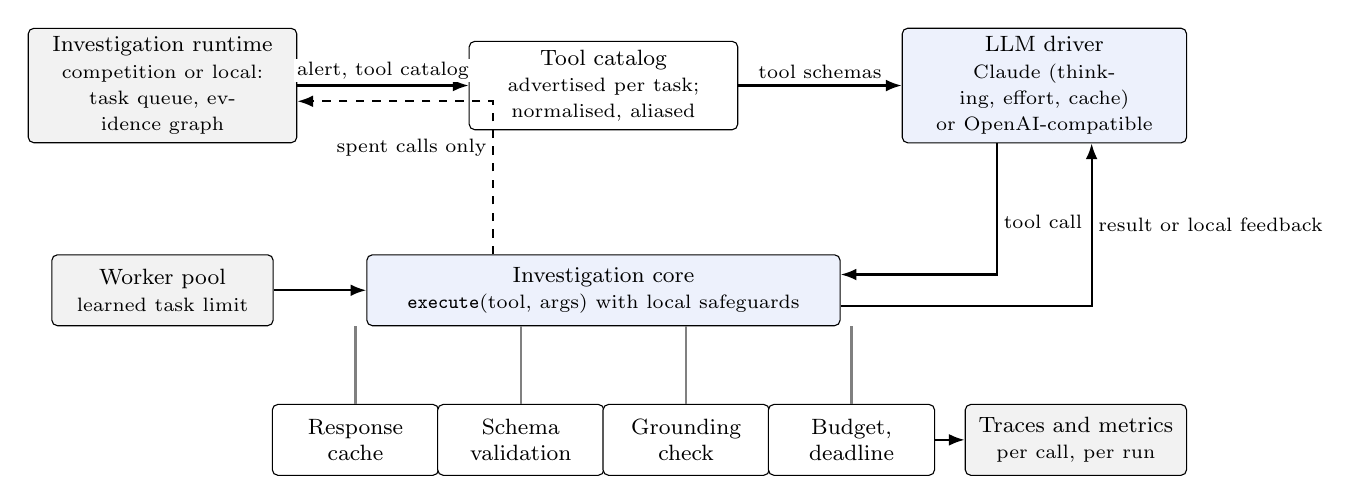
\begin{tikzpicture}[
  font=\footnotesize,
  box/.style={draw, rounded corners=2pt, align=center, text width=#1, inner sep=3pt, fill=white, minimum height=9mm},
  box/.default=30mm,
  arr/.style={-{Latex[length=2mm]}, thick},
  darr/.style={-{Latex[length=2mm]}, thick, dashed},
  lab/.style={font=\scriptsize, fill=white, inner sep=1pt}]

% top row
\node[box=32mm, fill=gray!10] (rt) at (0,0) {Investigation runtime\\{\scriptsize competition or local:}\\{\scriptsize task queue, evidence graph}};
\node[box=32mm] (cat) at (5.6,0) {Tool catalog\\{\scriptsize advertised per task;}\\{\scriptsize normalised, aliased}};
\node[box=34mm, fill=cA!8] (llm) at (11.2,0) {LLM driver\\{\scriptsize Claude (thinking, effort, cache)}\\{\scriptsize or OpenAI-compatible}};

% middle row
\node[box=26mm, fill=gray!10] (pool) at (0,-2.6) {Worker pool\\{\scriptsize learned task limit}};
\node[box=58mm, fill=cA!8] (inv) at (5.6,-2.6) {Investigation core\\{\scriptsize \tool{execute}(tool, args) with local safeguards}};
\node[box=26mm, fill=gray!10] (tr) at (11.6,-4.5) {Traces and metrics\\{\scriptsize per call, per run}};

% safeguards
\node[box=19mm] (c1) at (2.45,-4.5) {Response cache};
\node[box=19mm] (c2) at (4.55,-4.5) {Schema validation};
\node[box=19mm] (c3) at (6.65,-4.5) {Grounding check};
\node[box=19mm] (c4) at (8.75,-4.5) {Budget, deadline};
\foreach \c in {c1,c2,c3,c4} \draw[thick, gray] (\c.north) -- (\c.north |- inv.south);

% flows
\draw[arr] (rt) -- node[lab, above=1pt]{alert, tool catalog} (cat);
\draw[arr] (cat) -- node[lab, above=1pt]{tool schemas} (llm);
\draw[arr] ([xshift=-6mm]llm.south) |- node[lab, pos=0.3, right=1pt]{tool call} ([yshift=2mm]inv.east);
\draw[arr] ([yshift=-2mm]inv.east) -| node[lab, pos=0.75, right=1pt]{result or local feedback} ([xshift=6mm]llm.south);
\draw[darr] ([xshift=-14mm]inv.north) |- node[lab, pos=0.35, left=1pt]{spent calls only} ([yshift=-2mm]rt.east);
\draw[arr] (pool) -- (inv);
\draw[arr] (c4.east) -- (tr.west);
\end{tikzpicture}
\caption{Architecture. The runtime advertises a tool catalog with each task; the agent normalises it into
model tool definitions. Every tool call passes through the investigation core, whose local safeguards answer
repeated, malformed, ungrounded or over-budget calls without spending a runtime call; only the remaining calls
reach the runtime (dashed). A worker pool runs tasks in parallel up to the runtime's learned limit, and every
call and outcome is traced.}
\label{fig:arch}
\end{figure*}


\subsection{Catalog-driven tool interface}
\label{sec:catalog}
Each task observation carries the list of enabled tools with their argument schemas. The agent treats this
catalog as authoritative and builds the model's tool definitions from it on every task, rather than from a
hard-coded list, so changes to the runtime's tools need no code change. Schemas are normalised for portability
across model providers: local \texttt{\$ref} references are inlined, presentation-only keys are dropped,
\texttt{oneOf} alternatives that are distinguished by a constant discriminator are rewritten as the equivalent
\texttt{anyOf}, and the root is forced to be an object. When a catalog entry lacks a schema, the definition
falls back to the reference client's typed models. A JSON Schema validator (draft 2020-12) is compiled from
each normalised schema.

\subsection{Investigation method}
\label{sec:prompt}
The system prompt (Appendix~\ref{app:prompts}) encodes a hypothesis-driven method in three parts.
\emph{Method:} read the alert fully, form two or three competing hypotheses that always include a benign
explanation (administration, software update, backup, monitoring), and choose each call for the hypothesis it
can settle most decisively, usually by following relations outward from the trigger entity.
\emph{Spending discipline:} before every call, ask whether its answer could change the verdict or the artifact
list; never fetch what the alert or an earlier result already shows; request independent lookups together;
stop as soon as the verdict and the artifacts are supported. \emph{Submission guide:} which response kind fits
which entity (compromised host, used account, persistence, dropped file, control channel, observed entity),
and, for benign verdicts, which kinds of property prove legitimacy (valid signature, expected install path,
known management parent, documented service behaviour). The ablation \emph{no method} replaces this prompt
with a minimal one that states only the tool rules, close to the reference client's instructions.

\subsection{Local safeguards}
\label{sec:safeguards}
Every tool call the model issues is executed by Algorithm~\ref{alg:execute}. Its premise is that a runtime call
should be spent only when its result can be new information; everything else is answered locally, at no cost,
with feedback the model can act on.

\begin{algorithm}[t]
\caption{Execute a model-issued tool call}
\label{alg:execute}
\small
\begin{algorithmic}[1]
\Require tool $t$, arguments $x$; cache $\mathcal C$; rejected set $\mathcal R$; evidence corpus $\mathcal E$; calls spent $n$; hard budget $B$; finish-by time $T$
\State $x \gets \textsc{Unalias}(\textsc{NormaliseJSON}(x))$ \Comment{\S\ref{sec:alias}}
\State $k \gets (t, x \setminus \{\text{rationale}\})$
\If{$t\neq$ finish \textbf{and} $k\in\mathcal C$} \Return cached result \Comment{cache: no call spent}\EndIf
\If{$t\neq$ finish \textbf{and} ($n\ge B$ \textbf{or} now $\ge T$)} \Return ``submit now'' \Comment{budget, deadline}\EndIf
\If{$k\notin\mathcal R$}
  \If{$\textsc{Validate}(t,x)$ fails} $\mathcal R\gets\mathcal R\cup\{k\}$; \Return schema errors \EndIf
  \If{$t=$ finish \textbf{and} some cited id $\notin\mathcal E$} $\mathcal R\gets\mathcal R\cup\{k\}$; \Return ungrounded ids \EndIf
\EndIf
\State $y\gets$ \textsc{CallRuntime}$(t,x)$ with backoff on capacity refusals; $n\gets n+1$
\State $\mathcal E\gets\mathcal E\cup\{y\}$; \textbf{if} $y$ is not an error \textbf{then} $\mathcal C[k]\gets y$
\State \Return \textsc{Truncate}$(y)$
\end{algorithmic}
\end{algorithm}

\paragraph{Response cache} Identical calls (same tool, same arguments, ignoring the free-text rationale) are
answered from a cache with an explicit note that no call was spent. LLM agents re-request evidence they have
already seen, especially across long contexts; the cache makes that free.

\paragraph{Schema validation} Arguments are validated locally against the advertised schema. Invalid calls
receive the validator's messages instead of costing a runtime call. A call rejected locally is sent unchanged
if the model repeats it, so the runtime, not the agent, remains the authority on validity. A related
normalisation unwraps object-typed arguments that a model serialised as JSON strings.

\paragraph{Grounding check} Before a submission is sent, every entity and relation identifier it cites is
checked against the corpus of everything the alert and earlier tool results contained. Identifiers that never
appeared are reported back once (``use ids exactly as returned, or drop them''); an unchanged resubmission is
sent. This targets a failure specific to LLM agents: plausible but invented identifiers in an incident
response.

\paragraph{Budgets and deadline} After each batch of results the model sees the number of calls spent. Past a
soft budget it is told it is outside the efficient range; at a hard budget evidence calls are refused locally,
so the agent submits with what it has instead of exhausting the runtime's step limit and failing the task. An
optional deadline stops taking new tasks a few minutes before a cut-off and, shortly before it, allows only
submissions, so no task is left unsubmitted.

\subsection{Policy-compatible rationale fields}
\label{sec:alias}
The runtime requires a free-text field named \texttt{reasoning} on every evidence call and in the submission.
In early runs with a recent frontier model, the first request of every task was declined before any output,
with the refusal category \texttt{reasoning\_extraction}: the combination of a prompt asking the model to
``state its hypotheses'' and a required field called \texttt{reasoning} described as the ``investigation
trace'' read as a request to externalise the model's internal reasoning, which the model's usage policy
declines. The fix keeps the runtime contract intact. The instruction to state hypotheses was removed from
the first message (the method still asks the model to consider them), and the agent presents the field to the
model as
\texttt{purpose} (``one short sentence naming what this call checks'') and the submission's field as
\texttt{summary} (``a short incident summary''), and maps both back to \texttt{reasoning} before validation
and sending. The model's actual reasoning is read from its summarised thinking blocks. After the change, all
tasks of a mock run completed where all had previously been refused. We report this because any agent built
for a fixed runtime contract can meet the same conflict between the contract and a model provider's policies,
and because a field rename is enough to resolve it.

\subsection{Parallel execution with a learned limit}
\label{sec:parallel}
Budget-scored evaluations are often also time-boxed. The agent runs $W$ workers that each lease and investigate
tasks. Before leasing, a worker reserves a slot, so no more leases are attempted than the current limit allows.
If the runtime refuses a lease because of its active-task limit while other workers are busy, the pool lowers
its limit to the number of tasks in flight and the worker waits for a free slot; refusals while nothing else
runs are waited out with a bounded number of retries. Short operation-capacity or rate-limit refusals on tool
calls are retried with backoff; a refused call was not executed, so retrying spends nothing. One task's failure
is contained to that task.

\subsection{Model drivers}
\label{sec:drivers}
The Claude driver uses native tool use~\cite{anthropic_tooluse} with streaming, adaptive thinking (summarised
thinking is logged to the trace), an explicit effort level, automatic prompt caching~\cite{anthropic_promptcaching}
of the growing conversation prefix, and server-side fallback to another model on policy declines. Assistant turns are appended unchanged, so thinking blocks remain
valid for the next turn, and all results of a batch of parallel tool calls are returned in one message. An
OpenAI-compatible driver supports other providers; malformed tool-call JSON is answered locally without
spending a call. Both drivers nudge the model at most twice when it answers without a tool call, and abort the
task on a refusal. Every task produces a trace: each call with its stated purpose, its status
(\emph{ok}, \emph{cached}, \emph{refused locally}, \emph{error}, \emph{submitted}), the result, the summarised
reasoning, the submission, the runtime's score and token usage. Each run records its configuration and
aggregate metrics.

\section{The \bench Benchmark}
\label{sec:benchmark}

\bench turns public attack recordings into investigation tasks in the form defined in \S\ref{sec:problem}.
Fig.~\ref{fig:pipeline} shows the construction; Table~\ref{tab:tasks} lists the tasks.

% Benchmark construction pipeline (TikZ, vector). Included by sections/benchmark.tex.
\begin{figure}[t]
\centering
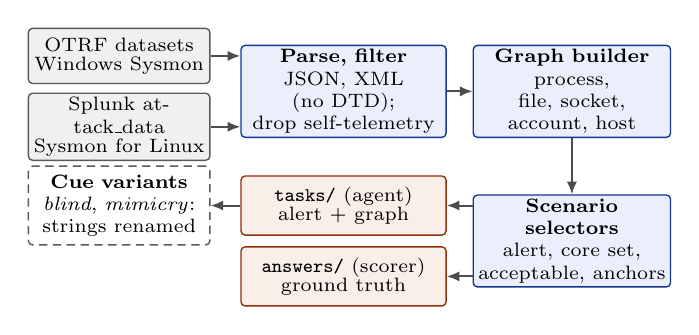
\begin{tikzpicture}[
  font=\scriptsize,
  >={Latex[length=1.6mm,width=1.3mm]},
  bx/.style={draw=cA!70!black, fill=cA!9, rounded corners=1.5pt, align=center,
             text width=#1, minimum height=10mm, inner sep=1.5pt, line width=0.5pt},
  bx/.default=24mm,
  src/.style={draw=black!65, fill=black!6, rounded corners=1.5pt, align=center,
              text width=22mm, minimum height=7mm, inner sep=1.5pt, line width=0.5pt},
  res/.style={draw=cB!75!black, fill=cB!9, rounded corners=1.5pt, align=center,
              text width=25mm, minimum height=7.5mm, inner sep=1.5pt, line width=0.5pt},
  arr/.style={->, line width=0.7pt, black!70}]
% row 1: public recordings -> parse -> graph
\node[src] (o) at (1.2,0.45) {OTRF datasets\\[-1pt]Windows Sysmon};
\node[src] (s) at (1.2,-0.45) {Splunk attack\_data\\[-1pt]Sysmon for Linux};
\node[bx=25mm] (p) at (4.05,0) {\textbf{Parse, filter}\\JSON, XML (no DTD);\\drop self-telemetry};
\node[bx] (g) at (6.95,0) {\textbf{Graph builder}\\process, file, socket,\\account, host};
% row 2: selectors -> tasks / answers -> cue variants
\node[bx] (sel) at (6.95,-1.9) {\textbf{Scenario selectors}\\alert, core set,\\acceptable, anchors};
\node[res] (t) at (4.05,-1.45) {\texttt{tasks/} (agent)\\[-1pt]alert + graph};
\node[res] (a) at (4.05,-2.35) {\texttt{answers/} (scorer)\\[-1pt]ground truth};
\node[bx=22mm, draw=black!65, fill=white, densely dashed] (v) at (1.2,-1.45)
  {\textbf{Cue variants}\\\emph{blind}, \emph{mimicry}:\\strings renamed};
\draw[arr] (o.east) -- (p.west |- o.east);
\draw[arr] (s.east) -- (p.west |- s.east);
\draw[arr] (p) -- (g);
\draw[arr] (g) -- (sel);
\draw[arr] (sel.west |- t.east) -- (t.east);
\draw[arr] (sel.west |- a.east) -- (a.east);
\draw[arr] (t) -- (v.east |- t.west);
\end{tikzpicture}
\caption{Construction of \bench from public recordings. Agents see only \texttt{tasks/}; the scorer uses
\texttt{answers/}. The cue-controlled variants rename strings in the tasks and keep graphs and answers.}
\label{fig:pipeline}
\end{figure}


\subsection{Sources and selection}
We use two practitioner corpora recorded with real endpoint sensors. OTRF Security-Datasets~\cite{otrf_securitydatasets}
(MIT licence) provides Windows Sysmon~\cite{microsoft_sysmon} and Security event logs captured while ATT\&CK techniques were executed
in a lab domain; Splunk attack\_data~\cite{splunk_attackdata} (Apache-2.0) provides, among other formats, Sysmon
for Linux~\cite{microsoft_sysmonforlinux} recordings from Ubuntu hosts in Splunk's Attack Range. We selected recordings
that (i) contain a complete process lineage for the activity, (ii) are small enough to package (each source
file is at most 34\,MB), and (iii) together cover distinct tactics: credential access, persistence, privilege
escalation, defence evasion, execution, impact and service stopping. We excluded recordings whose key step is
not observable in the telemetry (for instance, an authorised-keys write that the sensor did not capture) and
very large recordings. The result is \BenchWinMal{} malicious Windows and \BenchLinMal{} malicious Linux tasks
covering \BenchTechniques{} distinct ATT\&CK techniques, and \BenchWinBen{}+\BenchLinBen{} benign tasks.

\subsection{Graph construction}
A graph builder maps events to entities and relations using the runtime's type vocabulary
(Table~\ref{tab:types}). Sysmon process-creation events create a process entity keyed by its process GUID, a
parent entity from the parent fields, a process-creation relation and an executed-file relation; network,
image-load, process-access, file-create, file-delete, registry, pipe, DNS and WMI events add the corresponding
relations. Windows Security events add scheduled tasks and logons, and service-installation events add
services. Linux events use the Linux type names (\tool{linux\_process}, \tool{linux\_file}, \tool{linux\_user},
\tool{linux\_process\_create}). Users are linked to processes, processes to hosts, and repeated identical
relations (for example a beacon reconnecting from new ephemeral ports) are collapsed with a count and a
last-seen timestamp. Field values are copied from the events, capped at 600 characters. Event files are
treated as untrusted input: XML lines declaring a document type or entities are rejected.

\paragraph{Collector self-telemetry} The Linux recordings include the log forwarder's own checkpoint-file
writes under its installation directory, thousands per minute. These are artefacts of the collection pipeline,
not host activity, so file-create and file-delete events under that directory are dropped. The forwarder's
processes and network connections are kept as benign background. For the five recordings where this churn
dominated, it reduced graphs from roughly 11{,}000--33{,}500 entities to 50--150, leaving the real host
activity.

% Entity and relation types across the benchmark (generated).
\begin{table}[t]\centering\scriptsize
\caption{Entity and relation types across \bench (counts over all tasks).}
\label{tab:types}
\begin{tabular}{@{}lr@{\hspace{1.2em}}lr@{}}\toprule
Entity type & Count & Relation type & Count\\\midrule
\texttt{linux\_process} & 3338 & \texttt{runs\_process} & 3881\\
\texttt{windows\_file} & 1034 & \texttt{executed\_file} & 3176\\
\texttt{linux\_file} & 1006 & \texttt{linux\_process\_create} & 3147\\
\texttt{windows\_process} & 543 & \texttt{loaded\_image} & 1837\\
\texttt{registry\_key} & 361 & \texttt{accessed\_process} & 726\\
\texttt{network\_connection} & 297 & \texttt{deleted\_file} & 704\\
\texttt{linux\_user} & 42 & \texttt{created\_registry\_key} & 282\\
\texttt{host} & 23 & \texttt{connected\_to} & 205\\
\texttt{windows\_user} & 23 & \texttt{wrote\_file} & 142\\
\texttt{named\_pipe} & 7 & \texttt{set\_registry\_value} & 137\\
 & & \texttt{accepted\_connection\_from} & 122\\
 & & \texttt{logged\_on\_to} & 70\\
 & & \texttt{win\_process\_create} & 29\\
 & & \texttt{resolves\_to} & 7\\
 & & \texttt{connected\_to\_pipe} & 7\\
 & & \texttt{deleted\_registry\_key} & 4\\
\bottomrule\end{tabular}\end{table}


\subsection{Scenario design}
\paragraph{Malicious tasks} Each technique recording contains an operator's shell session (a Windows
\texttt{cmd.exe} or PowerShell, a Linux login shell) from which the technique was executed. The alert is what
a detection would raise on the key step, for example ``Process opened LSASS with full access'' for a
\texttt{rundll32} invoking the MiniDump export of \texttt{comsvcs.dll}, or ``Kernel module loaded with insmod''.
Alert texts describe the observable event without stating a verdict.

\paragraph{Benign tasks} Benign tasks are real background events from the same recordings that a naive
rule would flag. They include \texttt{svchost.exe} opening LSASS with access mask \texttt{0x1000}
(query-limited information, insufficient to read memory) next to the malicious dump that opened it with
\texttt{0x1FFFFF}; the Windows Time service writing \texttt{\textbackslash RunTime\textbackslash} values that
match a careless \texttt{\textbackslash Run} rule; and message-of-the-day scripts running discovery commands
as root at SSH login. Two pairs are \emph{twins}: in the Linux service recording, an operator stopping and
disabling a web service and the package manager starting it during installation raise the same alert
(``Service state changed by systemctl as root'') with opposite verdicts.

\subsection{Ground truth}
Ground truth is written as selectors over the graph (image name, command-line substring, path, user,
destination address, relation type) rather than as identifiers, and is rebuilt from the raw recordings on
every build. For a malicious task, the \emph{session root} is the operator shell above the trigger (its parent,
or the nearest ancestor with a given image). The core set $C$ contains the trigger and the session root, the
key commands, the artefacts that carry persistence or impact (the dump file, the Run-key value, the module
copied into \texttt{/lib/modules}, the script that wiped directories), the host, and the account to act on:
the session owner, plus the trigger's account unless it is the system account the session elevated to
(\texttt{SYSTEM}, \texttt{root}). The acceptable set $A^\star$ adds every process in the session and every
file, registry key, connection and process the session touched. For a benign task, the anchors are the trigger
and the entities that prove legitimacy, for example the parent that launched it (the package manager, the
login daemon) or the relation carrying the decisive property (the access mask), each with its real property
fields.

\subsection{Statistics and format}
Graphs have \BenchEntMin{}--\BenchEntMax{} entities (median \BenchEntMedian{}) and
\BenchRelMin{}--\BenchRelMax{} relations (median \BenchRelMedian{}), with \BenchEntTypes{} entity types and
\BenchRelTypes{} relation types overall. The benchmark is a single \BenchZipMB\,MB zip: a manifest, one task
file per task (alert and graph, no answers), one answer file per task, and the upstream licences. A local
runtime serves the tasks through the same client interface as the competition runtime and scores
submissions, so an agent runs on \bench unchanged.

\begin{table*}[t]\centering\scriptsize
\caption{The 21 tasks of \bench. Graph size is entities/relations; \emph{Core} is the number of core entities (malicious) or legitimacy anchors (benign) in the ground truth.}
\label{tab:tasks}
\begin{tabular}{@{}lllllrr@{}}\toprule
Task & OS & Verdict & ATT\&CK & Alert title & Graph & Core\\\midrule
\texttt{lsass-dump-comsvcs} & Win & malicious & T1003.001 & Process opened LSASS with full access & 88/115 & 5\\
\texttt{logon-script-persistence} & Win & malicious & T1037.001 & User environment registry value written by reg.exe & 47/75 & 6\\
\texttt{service-binpath-hijack} & Win & malicious & T1543.003 & Service configuration changed with sc.exe & 157/219 & 6\\
\texttt{hta-startup-folder} & Win & malicious & T1218.005 & mshta.exe executed an HTA file & 338/717 & 6\\
\texttt{firewall-rule-added} & Win & malicious & T1562.004 & Inbound firewall rule added from the command line & 174/365 & 4\\
\texttt{python-http-server} & Win & malicious & T1059 & Interpreter from a user profile started a network service & 300/633 & 6\\
\texttt{bits-download} & Win & malicious & T1197 & BITS transfer job started from the command line & 186/247 & 4\\
\texttt{run-key-and-beacon} & Win & malicious & T1547.001 & Autostart Run key value set by PowerShell & 74/87 & 5\\
\texttt{lsass-query-by-svchost} & Win & benign & - & Process opened a handle to LSASS & 186/247 & 2\\
\texttt{w32time-runtime-key} & Win & benign & - & Registry value written under a path matching '\textbackslash{}Run' & 300/633 & 3\\
\texttt{gpsvc-service-host} & Win & benign & - & New service host process started as SYSTEM & 174/365 & 2\\
\texttt{linux-shadow-read} & Lin & malicious & T1003.008 & Credential file read by a script run with sudo & 50/76 & 6\\
\texttt{linux-wiper-shred} & Lin & malicious & T1485 & shred overwrote a system directory & 317/672 & 7\\
\texttt{linux-kernel-module} & Lin & malicious & T1547.006 & Kernel module loaded with insmod & 78/142 & 6\\
\texttt{linux-account-created} & Lin & malicious & T1136.001 & Local account created & 76/127 & 5\\
\texttt{linux-sudoers-nopasswd} & Lin & malicious & T1548.003 & Passwordless sudo rule written & 141/245 & 5\\
\texttt{linux-ld-preload-hijack} & Lin & malicious & T1574.006 & Freshly compiled binary executed as root from a home directory & 150/265 & 8\\
\texttt{linux-service-stopped} & Lin & malicious & T1489 & Service state changed by systemctl as root & 1602/3951 & 5\\
\texttt{linux-dpkg-service-start} & Lin & benign & - & Service state changed by systemctl as root & 1602/3951 & 3\\
\texttt{linux-motd-discovery} & Lin & benign & - & Session discovery command run as root & 317/672 & 3\\
\texttt{linux-motd-tmp-cleanup} & Lin & benign & - & Files deleted by rm as root & 317/672 & 3\\
\bottomrule\end{tabular}\end{table*}


\section{Experimental Setup}
\label{sec:experiments}

\subsection{Model and agent configuration}
All runs use Claude Opus 5.5 (\texttt{claude-opus-5-5}) through the Anthropic Messages API with adaptive
thinking and effort level \emph{high}, a soft budget of 12 tool calls, a hard cap of 30, at most 45 model turns
per task, and tool results truncated at 24{,}000 characters. Four tasks run in parallel. The local runtime
serves \bench through the same client interface as the competition runtime and scores each submission with
the scorer of \S\ref{sec:problem}. Like a server, it checks every call's arguments against the tool schema
and answers a non-conforming call with an error; the call still counts. This fixes what the \emph{no
validation} ablation measures: malformed calls cost runtime calls instead of being caught locally. The optimum $n^\star$ is set per task when the task is defined, as the
length of a minimal investigation path to the ground truth (2 to 5 calls, including the submission).

\subsection{Configurations}
The \emph{full} configuration enables every component of \S\ref{sec:method}. Five ablations each switch off
one component:
\begin{itemize}
\item \emph{no cache}: repeated calls are sent to the runtime again;
\item \emph{no validation}: arguments are not checked locally;
\item \emph{no grounding}: submissions citing unseen identifiers are sent without warning;
\item \emph{no budget}: no call-count feedback and no hard cap (the turn limit still applies);
\item \emph{no method}: the investigation-method prompt is replaced by a minimal prompt stating only the tool
rules (Appendix~\ref{app:prompts}).
\end{itemize}
Because LLM outputs vary between runs, each configuration is run three times on all 21 tasks, and we report
means with standard deviations across repeats. A single command runs the full configuration followed by the
five ablations on the same tasks. The first repeat was made with \bench v1.0 and rescored on v1.1
(\S\ref{sec:benchmark}); since the graphs are identical and scores depend only on the submission and the
number of calls, rescoring from the stored traces is exact. One run is excluded: in the first repeat of
\emph{no validation}, a malformed argument crashed the v1.0 runtime and aborted a task, which a schema-checking
runtime would have rejected instead; that configuration therefore has two repeats.

\subsection{Metrics}
Per task we record quality $Q$, efficiency $E$, reward $R$, tool calls spent, calls answered by the cache,
calls refused locally, wall-clock time and tokens (input, output, cache reads). Aggregates per configuration:
mean $Q$, $E$, $R$ and calls; verdict accuracy; the false-positive rate (benign tasks judged malicious) and the
false-negative rate (malicious tasks judged benign); each also broken down by operating system and by expected
verdict. All figures in \S\ref{sec:results} are regenerated from the run folders by a script in the release.

\subsection{Pilot}
Before the Linux tasks existed, we ran the full configuration once on the \ResPilotTasks{} Windows tasks (then
\bench v0). The pilot used the same model and prompt and is reported as scored at the time, with the v1.0
ground truth. The revision to v1.1 leaves the Windows malicious ground truth unchanged; the three Windows benign
tasks gained small neutral sets (one or two lineage ids each), so the pilot's benign quality can only be
understated.

\subsection{Implementation and testing}
The agent is written in Python and installs into the competition's public reference client. Its test suite
(25 tests, in addition to the reference client's own) covers the catalog normalisation, every safeguard and
ablation switch, the field aliasing, parallel execution against a simulated runtime with a task limit
(including through the reference client's own transport layer), deadline handling, the graph builder on
Windows and Linux events, scoring and the ground-truth rules, the runtime's rejection of malformed calls, the
benchmark pack round trip, offline rescoring and a scripted run on the real recordings.

\section{Results and Analysis}
\label{sec:results}

\subsection{Pilot: Windows tasks}
\label{sec:pilot}
Table~\ref{tab:pilot} reports the pilot on the \ResPilotTasks{} Windows tasks. All tasks completed and every
verdict was correct (accuracy \ResPilotAccuracy{}): the eight attacks were judged malicious and the three
benign look-alikes benign, so the false-positive and false-negative rates were both zero. Mean quality was
\ResPilotQuality{}, mean efficiency \ResPilotEfficiency{} and mean reward \ResPilotReward{}, with
\ResPilotCalls{} tool calls per task (range \ResPilotMinCalls{}--\ResPilotMaxCalls{}). The whole run took
\ResPilotWall\,s of wall-clock time with four tasks in parallel.

\begin{table}[t]\centering\footnotesize
\caption{Pilot run on the 11 Windows tasks (Claude Opus 5.5, effort \emph{high}, full configuration). Quality is 0 for a wrong verdict, so every verdict here was correct.}
\label{tab:pilot}
\resizebox{\columnwidth}{!}{%
\begin{tabular}{@{}llrrrr@{}}\toprule
Task & Expected & Quality & Effic. & Reward & Calls\\\midrule
\texttt{logon-script-persistence} & malicious & 0.917 & 0.714 & 0.864 & 7\\
\texttt{lsass-dump-comsvcs} & malicious & 1.000 & 0.714 & 0.943 & 7\\
\texttt{service-binpath-hijack} & malicious & 0.922 & 0.600 & 0.849 & 10\\
\texttt{hta-startup-folder} & malicious & 0.922 & 0.500 & 0.830 & 12\\
\texttt{firewall-rule-added} & malicious & 0.887 & 0.667 & 0.828 & 6\\
\texttt{bits-download} & malicious & 0.929 & 0.800 & 0.891 & 5\\
\texttt{run-key-and-beacon} & malicious & 0.908 & 0.625 & 0.840 & 8\\
\texttt{lsass-query-by-svchost} & benign & 1.000 & 1.000 & 1.000 & 3\\
\texttt{python-http-server} & malicious & 0.922 & 0.455 & 0.822 & 11\\
\texttt{w32time-runtime-key} & benign & 1.000 & 0.750 & 0.950 & 4\\
\texttt{gpsvc-service-host} & benign & 0.850 & 0.429 & 0.753 & 7\\
\midrule
Mean & & 0.933 & 0.659 & 0.870 & 7.27\\
\bottomrule\end{tabular}}\end{table}


\paragraph{Where reward is lost (RQ2)} Since $R=Q(0.8+0.2E)$, the gap between the mean reward and its maximum
of 1 decomposes into a quality part, $\overline{1-Q}=0.068$, and an efficiency part,
$\overline{0.2\,Q(1-E)}=0.063$. Efficiency therefore costs almost as much as imperfect artifacts.
Fig.~\ref{fig:pilotcalls} shows why: the agent used 80 tool calls against a target of 49 (the sum of
$n^\star+1$), and 10 of 11 tasks exceeded their target. The largest overruns were the HTA execution (12 calls
against a target of 6), the Python HTTP server (11 against 5) and the service-configuration change (10 against
6), all multi-step chains in which the agent fetched relations one at a time. Benign tasks were cheaper
(4.7 calls on average, efficiency 0.73) than malicious ones (8.3 calls, efficiency 0.63), except the Group
Policy service host (7 calls against a target of 3), where the agent kept collecting evidence after the parent
process alone settled the question.

\paragraph{Quality} Quality was 1.0 on three tasks and at least 0.85 on all. With a correct verdict, the
score leaves only two ways to lose quality: for malicious tasks, missing core entities or naming entities
outside the acceptable set; for benign tasks, citing only some anchors or non-decisive fields. The per-call
traces of the study runs attribute these losses per task.

% Pilot: tool calls per task against the optimal count (pgfplots, reads data/pilot_per_task.csv).
\begin{figure}[t]
\centering
\begin{tikzpicture}
\begin{axis}[
  xbar, bar width=4pt, width=0.62\columnwidth, height=7.2cm,
  xmin=0, xmax=13, xlabel={Tool calls}, xmajorgrids, grid style={gray!25},
  symbolic y coords={gpsvc-service-host,w32time-runtime-key,lsass-query-by-svchost,python-http-server,run-key-and-beacon,bits-download,firewall-rule-added,hta-startup-folder,service-binpath-hijack,lsass-dump-comsvcs,logon-script-persistence},
  ytick=data, yticklabel style={font=\tiny\ttfamily}, tick label style={font=\scriptsize},
  legend style={font=\scriptsize, at={(0.98,0.02)}, anchor=south east, draw=gray!40},
  enlarge y limits=0.06,
]
\addplot[fill=cA, draw=none] table[col sep=comma, x=calls, y=task] {data/pilot_per_task.csv};
\addplot[fill=cB, draw=none] table[col sep=comma, x expr=\thisrow{optimal}+1, y=task] {data/pilot_per_task.csv};
\legend{Used, Optimal + 1}
\end{axis}
\end{tikzpicture}
\caption{Pilot run: tool calls used per task against the efficiency target (optimal + 1, at which efficiency
reaches 1). Every verdict was correct; the gap between the bars is the efficiency loss.}
\label{fig:pilotcalls}
\end{figure}


\subsection{Full study and ablation (RQ1, RQ3, RQ4)}
\label{sec:study}
\ifnum\ResStudyAvailable=1
Table~\ref{tab:ablation} reports the full configuration and the five ablations over \ResStudyTasks{} tasks
with \ResStudyRepeats{} repeats per configuration; Table~\ref{tab:effects} gives paired task-level effects,
Table~\ref{tab:breakdown} a breakdown by operating system and expected verdict, Table~\ref{tab:pertask} the
per-task matrix and Table~\ref{tab:safeguards} what happened at the tool interface. Repeat~1 was rescored from
v1.0 (\S\ref{sec:experiments}); all \ResPairedRepeats{} repeats have per-task results and traces.

\begin{table*}[t]\centering\footnotesize
\caption{Ablation study on SOCGraph-21. Each row turns off one component of the full agent; values are means over repeated runs ($\pm$ standard deviation when $n>1$). $\Delta$Reward is relative to the full configuration on the same tasks.}
\label{tab:ablation}
\begin{tabular}{@{}l r rrrrrrr r@{}}\toprule
Configuration & $n$ & Quality & Efficiency & Reward & Verdict acc. & FPR & FNR & Calls/task & $\Delta$Reward\\\midrule
full & 3 & 0.836\,$\pm$\,0.013 & 0.626\,$\pm$\,0.019 & 0.775\,$\pm$\,0.012 & 0.968\,$\pm$\,0.027 & 0.000\,$\pm$\,0.000 & 0.044\,$\pm$\,0.039 & 8.22\,$\pm$\,0.22 & --\\
no cache & 3 & 0.866\,$\pm$\,0.005 & 0.610\,$\pm$\,0.007 & 0.799\,$\pm$\,0.005 & 1.000\,$\pm$\,0.000 & 0.000\,$\pm$\,0.000 & 0.000\,$\pm$\,0.000 & 8.43\,$\pm$\,0.08 & +0.023\\
no validation & 2 & 0.872\,$\pm$\,0.003 & 0.618\,$\pm$\,0.001 & 0.805\,$\pm$\,0.002 & 1.000\,$\pm$\,0.000 & 0.000\,$\pm$\,0.000 & 0.000\,$\pm$\,0.000 & 8.45\,$\pm$\,0.03 & +0.029\\
no grounding & 3 & 0.843\,$\pm$\,0.027 & 0.610\,$\pm$\,0.007 & 0.779\,$\pm$\,0.023 & 0.968\,$\pm$\,0.027 & 0.000\,$\pm$\,0.000 & 0.044\,$\pm$\,0.039 & 8.49\,$\pm$\,0.19 & +0.004\\
no budget & 3 & 0.871\,$\pm$\,0.007 & 0.608\,$\pm$\,0.008 & 0.802\,$\pm$\,0.006 & 1.000\,$\pm$\,0.000 & 0.000\,$\pm$\,0.000 & 0.000\,$\pm$\,0.000 & 8.75\,$\pm$\,0.29 & +0.027\\
no method & 3 & 0.830\,$\pm$\,0.026 & 0.432\,$\pm$\,0.009 & 0.737\,$\pm$\,0.022 & 0.937\,$\pm$\,0.027 & 0.000\,$\pm$\,0.000 & 0.089\,$\pm$\,0.038 & 11.70\,$\pm$\,0.28 & -0.038\\
\bottomrule\end{tabular}\end{table*}

\begin{table*}[t]\centering\footnotesize
\caption{Paired effect of each ablation against the full agent: per-task difference, averaged over the 2 repeats with per-task results, with a bootstrap 95\% interval over the tasks (10{,}000 resamples). The third column leaves out the task whose verdict was unstable. \emph{More calls}: tasks on which the ablation used more calls than the full agent, of those where the number differed.}
\label{tab:effects}
\begin{tabular}{@{}lrrrr@{}}\toprule
Configuration & $\Delta$Reward [95\% CI] & excl.\ \texttt{linux-service-stopped} & $\Delta$Calls [95\% CI] & More calls\\\midrule
no cache & +0.017 [-0.016, +0.064] & -0.004 [-0.020, +0.009] & +0.17 [-0.29, +0.62] & 9/15\\
no validation & +0.024 [-0.004, +0.070] & +0.004 [-0.006, +0.015] & +0.17 [-0.14, +0.50] & 9/15\\
no grounding & +0.007 [-0.003, +0.018] & +0.005 [-0.005, +0.016] & +0.19 [-0.31, +0.76] & 6/12\\
no budget & +0.022 [-0.008, +0.068] & +0.001 [-0.011, +0.012] & +0.31 [-0.31, +1.02] & 9/15\\
no method & -0.031 [-0.078, +0.008] & -0.013 [-0.044, +0.015] & +3.57 [+2.43, +4.79] & 20/20\\
\bottomrule\end{tabular}\end{table*}

% Ablation: quality and efficiency per configuration (pgfplots, reads data/runs.csv).
% Drawn only when the study results exist (\ResStudyAvailable = 1).
\pgfplotstableread[col sep=comma]{data/runs.csv}\ablationruns
\begin{figure}[t]
\centering
\begin{tikzpicture}
\begin{axis}[
  ybar, bar width=6pt, width=0.95\columnwidth, height=5.4cm,
  ymin=0, ymax=1.05, ylabel={Mean over tasks}, ymajorgrids, grid style={gray!25},
  xticklabels from table={\ablationruns}{configuration}, xtick=data,
  xticklabel style={font=\scriptsize, rotate=25, anchor=north east},
  tick label style={font=\scriptsize}, legend style={font=\scriptsize, at={(0.5,1.02)}, anchor=south, legend columns=2, draw=none},
]
\addplot[fill=cA, draw=none, error bars/.cd, y dir=both, y explicit]
  table[x expr=\coordindex, y=mean_quality, y error=mean_quality_sd] {\ablationruns};
\addplot[fill=cB, draw=none, error bars/.cd, y dir=both, y explicit]
  table[x expr=\coordindex, y=mean_efficiency, y error=mean_efficiency_sd] {\ablationruns};
\legend{Quality, Efficiency}
\end{axis}
\end{tikzpicture}
\caption{Mean quality and efficiency per configuration (error bars: standard deviation over repeats).}
\label{fig:ablation}
\end{figure}


\paragraph{Effectiveness (RQ1)} The full agent reached reward \ResFullReward{}\,$\pm$\,\ResFullRewardSd{},
quality \ResFullQuality{} and verdict accuracy \ResFullAccuracy{}. No configuration judged a benign task
malicious in any run, so the false-positive rate was zero throughout. The full agent's verdict errors
(\ResFullVerdictErrors{}) were both on \texttt{linux-service-stopped}, the malicious member of the twin pair.
Across all configurations this task was cleared in 7 of the 17 runs, while its benign twin, with the same
alert, was judged correctly in all 17. The traces show why: in each erroneous run the agent observed that the
operator ran \texttt{status} and \texttt{restart} on the service seconds after stopping it, and concluded that
nothing was kept down. That sequence is the cleanup step of the recorded test, so the benign reading is
defensible from the telemetry alone; the label follows the recording's intent. The only other error was one
malicious Windows task (\texttt{firewall-rule-added}) cleared without the method prompt.

\paragraph{Platforms and verdict classes (RQ4)} Quality was \ResFullWinQuality{} on Windows tasks and
\ResFullLinQuality{} on Linux tasks. The traces show two systematic patterns that cost quality on both
platforms, more on Linux. (i) \emph{Hosts named by hostname.} Of the \TrAllMalSubs{} correct malicious
submissions, \TrAllHostByName{} named the host to isolate by its hostname instead of its entity id, which
the scorer counts as a missed core entity and an unrelated citation; only \TrAllHostById{} used the id.
(ii) \emph{Lineage relations and the session root.} On the benign Linux tasks the agent cited the
process-creation relations along the trigger's lineage, which v1.1 does not count as neutral, and stopped at
the script that explains the activity (the MOTD script, the package's post-installation script) instead of
citing the session root above it (\texttt{sshd}, \texttt{dpkg}). Hence the constant $Q=0.708$ on
\texttt{linux-dpkg-service-start} and \texttt{linux-motd-discovery}: two of three anchors and two relation
citations outside $\mathcal L\cup N$.

\begin{table}[t]\centering\footnotesize
\caption{Scoring sensitivity: mean quality of the full agent's 63 submissions rescored under alternative rules (no new model calls).}
\label{tab:sensitivity}
\resizebox{\columnwidth}{!}{%
\begin{tabular}{@{}lrrrrr@{}}\toprule
Scoring rule & All & Windows & Linux & Malicious & Benign\\\midrule
Official (v1.1) & 0.836 & 0.930 & 0.733 & 0.837 & 0.836\\
+ lineage relations neutral & 0.855 & 0.934 & 0.769 & 0.837 & 0.903\\
+ hostnames accepted & 0.876 & 0.973 & 0.769 & 0.892 & 0.836\\
+ both & 0.895 & 0.977 & 0.806 & 0.892 & 0.903\\
\bottomrule\end{tabular}}\end{table}


Table~\ref{tab:sensitivity} rescores the full agent's \TrFullSubmissions{} submissions under alternative rules,
without new model calls. Accepting hostnames raises Windows quality from \SensOfficialWindows{} to
\SensHostnamesWindows{}; treating lineage relations as neutral raises benign quality from \SensOfficialBenign{}
to \SensRelationsBenign{}; with both, overall quality rises from \SensOfficialAll{} to \SensBothAll{} and Linux
from \SensOfficialLinux{} to \SensBothLinux{}. We keep the official scorer, which is fixed and released; the
table shows how much of the measured gap reflects identifier discipline and evidence style rather than wrong
conclusions. The Linux gap that remains comes from the twin errors and from tasks where the agent drew the
operator session differently from the ground truth: on \texttt{linux-sudoers-nopasswd} it treated the script
that wrote the rule, not the login shell above it, as the session root, and named \texttt{root} rather than the
operator account.

\paragraph{Efficiency and where reward is lost (RQ2)} The full agent used \ResFullCalls{} calls per task
against a mean target $n^\star+1$ of 4.6, and exceeded the target in 58 of 63 task runs. The reward gap
decomposes into a quality part, $1-\overline{Q}=0.164$, and an efficiency part,
$\overline{Q}-\overline{R}=0.061$; on the full benchmark, unlike the Windows-only pilot, quality is the larger
loss. A task took \TrFullModelCalls{} model calls on average, with about \TrFullOutTok{} output tokens and
\TrFullCacheReadTok{} prompt tokens read from the cache; uncached input was negligible because the system
prompt and tool definitions were cached. The hard cap of 30 calls was never reached (at most 22 in any run).

\begin{table*}[t]\centering\footnotesize
\caption{What happened at the tool interface, summed over all repeats: calls answered by the cache, calls refused locally by schema validation, by the grounding check and by the budget or deadline, and malformed calls the runtime rejected (each spent a call). Tokens and model calls are means per task; \emph{Host by id/name}: correct malicious submissions naming the host by its entity id, or by its hostname.}
\label{tab:safeguards}
\begin{tabular}{@{}lrrrrrrrrrr@{}}\toprule
Configuration & Tasks & Cache & Valid. & Ground. & Budget & Runtime rej. & Output tok. & Cache-read tok. & Model calls & Host by id/name\\\midrule
full & 63 & 0 & 5 & 1 & 0 & 0 & 1{,}550 & 35{,}544 & 5.79 & 4/29\\
no cache & 63 & 0 & 4 & 1 & 0 & 0 & 1{,}547 & 38{,}281 & 5.86 & 7/28\\
no validation & 42 & 0 & 0 & 0 & 0 & 5 & 1{,}556 & 37{,}808 & 5.81 & 6/20\\
no grounding & 63 & 0 & 8 & 0 & 0 & 0 & 1{,}576 & 37{,}146 & 5.73 & 7/28\\
no budget & 63 & 1 & 7 & 0 & 0 & 0 & 1{,}627 & 40{,}162 & 6.11 & 8/29\\
no method & 63 & 0 & 12 & 0 & 0 & 0 & 2{,}024 & 32{,}241 & 6.57 & 16/10\\
\bottomrule\end{tabular}\end{table*}


\paragraph{Ablation (RQ3): the method prompt} Replacing the investigation-method prompt with the minimal prompt
is the only ablation with a consistent effect. The agent then used \ResNoMethodPairedCalls{} calls per task more
(95\% CI \ResNoMethodPairedCallsCI{}), more on \ResNoMethodMoreCalls{} of the \ResNoMethodCallsDiffer{} tasks
where the count differed (sign test \ResNoMethodCallsSignP{}), and efficiency fell from \ResFullEfficiency{} to
\ResNoMethodEfficiency{}. The paired change in mean reward was \ResNoMethodPairedReward{} (95\% CI
\ResNoMethodPairedRewardCI{}).
Quality did not fall (\ResNoMethodQuality{} against \ResFullQuality{}), for a reason the traces make visible:
the method prompt tells the agent not to look up the host named in the alert, so the full agent rarely held the
host's entity id (\TrFullHostById{} of \TrFullMalSubs{} correct malicious submissions used it, against
\TrNoMethodHostById{} of \TrNoMethodMalSubs{} without the method). An efficiency instruction thus cost quality
through the interface, offsetting what the method gains elsewhere. Without the method the agent also sent more
malformed calls (\TrNoMethodValidation{} refused by validation, against \TrFullValidation{}) and used about
30\% more output tokens.

\paragraph{Ablation (RQ3): the local safeguards} Switching off the cache, validation, grounding check or budget
produced no measurable change. Three of these ablations score about 0.02--0.03 above the full agent in mean
reward, but the difference is the twin task: the full agent cleared \texttt{linux-service-stopped} in two of
three repeats, and each miss removes about 0.04 from the mean over 21 tasks. Leaving that task out, every
paired difference lies within $\pm0.004$ and every interval contains zero (Table~\ref{tab:effects}). The
per-configuration error counts on that task are consistent with one common rate: with the pooled 7 errors in 17
runs, two or more errors in three runs has probability of about 0.37 and none about 0.20.

Table~\ref{tab:safeguards} shows why the safeguards had nothing to win. In \TrFullTasks{} full-agent tasks the
cache answered \TrFullCache{} calls, validation refused \TrFullValidation{} malformed calls (a search query
shorter than the schema's minimum, a submission serialised as an invalid JSON string), the grounding check
fired \TrFullGrounding{} time (an invented host identifier, \texttt{host-workstation5}, which the agent then
dropped) and the budget never refused a call. Without validation, the same kinds of malformed call reached the
runtime \TrNoValidationRuntimeSchema{} times in 42 tasks and were rejected there, each costing a call: about
0.1 calls per task, too few to move efficiency. The grounding check also missed the most frequent identifier
error: it accepts any string that occurred in the evidence, and hostnames do occur there. A check that accepts
only values seen in identifier fields would have flagged all \TrAllHostByName{} hostname citations.
\else
The full study runs every configuration of \S\ref{sec:experiments} three times on all 21 tasks. Its results
are generated into Tables~\ref{tab:ablation}--\ref{tab:pertask} and a comparison figure by the release
script from the run folders, and this subsection will report them.
\fi

\ifnum\ResStudyAvailable=0
\begin{table*}[t]\centering\footnotesize
\caption{Ablation study on SOCGraph-21. Each row turns off one component of the full agent; values are means over repeated runs ($\pm$ standard deviation when $n>1$). $\Delta$Reward is relative to the full configuration on the same tasks.}
\label{tab:ablation}
\begin{tabular}{@{}l r rrrrrrr r@{}}\toprule
Configuration & $n$ & Quality & Efficiency & Reward & Verdict acc. & FPR & FNR & Calls/task & $\Delta$Reward\\\midrule
full & 3 & 0.836\,$\pm$\,0.013 & 0.626\,$\pm$\,0.019 & 0.775\,$\pm$\,0.012 & 0.968\,$\pm$\,0.027 & 0.000\,$\pm$\,0.000 & 0.044\,$\pm$\,0.039 & 8.22\,$\pm$\,0.22 & --\\
no cache & 3 & 0.866\,$\pm$\,0.005 & 0.610\,$\pm$\,0.007 & 0.799\,$\pm$\,0.005 & 1.000\,$\pm$\,0.000 & 0.000\,$\pm$\,0.000 & 0.000\,$\pm$\,0.000 & 8.43\,$\pm$\,0.08 & +0.023\\
no validation & 2 & 0.872\,$\pm$\,0.003 & 0.618\,$\pm$\,0.001 & 0.805\,$\pm$\,0.002 & 1.000\,$\pm$\,0.000 & 0.000\,$\pm$\,0.000 & 0.000\,$\pm$\,0.000 & 8.45\,$\pm$\,0.03 & +0.029\\
no grounding & 3 & 0.843\,$\pm$\,0.027 & 0.610\,$\pm$\,0.007 & 0.779\,$\pm$\,0.023 & 0.968\,$\pm$\,0.027 & 0.000\,$\pm$\,0.000 & 0.044\,$\pm$\,0.039 & 8.49\,$\pm$\,0.19 & +0.004\\
no budget & 3 & 0.871\,$\pm$\,0.007 & 0.608\,$\pm$\,0.008 & 0.802\,$\pm$\,0.006 & 1.000\,$\pm$\,0.000 & 0.000\,$\pm$\,0.000 & 0.000\,$\pm$\,0.000 & 8.75\,$\pm$\,0.29 & +0.027\\
no method & 3 & 0.830\,$\pm$\,0.026 & 0.432\,$\pm$\,0.009 & 0.737\,$\pm$\,0.022 & 0.937\,$\pm$\,0.027 & 0.000\,$\pm$\,0.000 & 0.089\,$\pm$\,0.038 & 11.70\,$\pm$\,0.28 & -0.038\\
\bottomrule\end{tabular}\end{table*}

\begin{table*}[t]\centering\footnotesize
\caption{Paired effect of each ablation against the full agent: per-task difference, averaged over the 2 repeats with per-task results, with a bootstrap 95\% interval over the tasks (10{,}000 resamples). The third column leaves out the task whose verdict was unstable. \emph{More calls}: tasks on which the ablation used more calls than the full agent, of those where the number differed.}
\label{tab:effects}
\begin{tabular}{@{}lrrrr@{}}\toprule
Configuration & $\Delta$Reward [95\% CI] & excl.\ \texttt{linux-service-stopped} & $\Delta$Calls [95\% CI] & More calls\\\midrule
no cache & +0.017 [-0.016, +0.064] & -0.004 [-0.020, +0.009] & +0.17 [-0.29, +0.62] & 9/15\\
no validation & +0.024 [-0.004, +0.070] & +0.004 [-0.006, +0.015] & +0.17 [-0.14, +0.50] & 9/15\\
no grounding & +0.007 [-0.003, +0.018] & +0.005 [-0.005, +0.016] & +0.19 [-0.31, +0.76] & 6/12\\
no budget & +0.022 [-0.008, +0.068] & +0.001 [-0.011, +0.012] & +0.31 [-0.31, +1.02] & 9/15\\
no method & -0.031 [-0.078, +0.008] & -0.013 [-0.044, +0.015] & +3.57 [+2.43, +4.79] & 20/20\\
\bottomrule\end{tabular}\end{table*}

\fi
\begin{table*}[t]\centering\footnotesize
\caption{Quality and verdict accuracy by platform and by expected verdict, over the repeats with per-task results (mean $\pm$ standard deviation across repeats).}
\label{tab:breakdown}
\begin{tabular}{@{}l rrrrrrrr@{}}\toprule
Configuration & \multicolumn{2}{c}{Windows} & \multicolumn{2}{c}{Linux} & \multicolumn{2}{c}{Malicious} & \multicolumn{2}{c}{Benign}\\
\cmidrule(lr){2-3}\cmidrule(lr){4-5}\cmidrule(lr){6-7}\cmidrule(lr){8-9}
 & Qual. & Acc. & Qual. & Acc. & Qual. & Acc. & Qual. & Acc.\\\midrule
full & 0.930\,$\pm$\,0.017 & 1.00\,$\pm$\,0.00 & 0.733\,$\pm$\,0.034 & 0.93\,$\pm$\,0.06 & 0.837\,$\pm$\,0.020 & 0.96\,$\pm$\,0.04 & 0.836\,$\pm$\,0.004 & 1.00\,$\pm$\,0.00\\
no cache & 0.938\,$\pm$\,0.012 & 1.00\,$\pm$\,0.00 & 0.787\,$\pm$\,0.010 & 1.00\,$\pm$\,0.00 & 0.879\,$\pm$\,0.008 & 1.00\,$\pm$\,0.00 & 0.833\,$\pm$\,0.004 & 1.00\,$\pm$\,0.00\\
no validation & 0.941\,$\pm$\,0.009 & 1.00\,$\pm$\,0.00 & 0.795\,$\pm$\,0.005 & 1.00\,$\pm$\,0.00 & 0.885\,$\pm$\,0.002 & 1.00\,$\pm$\,0.00 & 0.838\,$\pm$\,0.003 & 1.00\,$\pm$\,0.00\\
no grounding & 0.942\,$\pm$\,0.005 & 1.00\,$\pm$\,0.00 & 0.735\,$\pm$\,0.052 & 0.93\,$\pm$\,0.06 & 0.845\,$\pm$\,0.036 & 0.96\,$\pm$\,0.04 & 0.840\,$\pm$\,0.007 & 1.00\,$\pm$\,0.00\\
no budget & 0.932\,$\pm$\,0.007 & 1.00\,$\pm$\,0.00 & 0.803\,$\pm$\,0.010 & 1.00\,$\pm$\,0.00 & 0.887\,$\pm$\,0.007 & 1.00\,$\pm$\,0.00 & 0.831\,$\pm$\,0.009 & 1.00\,$\pm$\,0.00\\
no method & 0.920\,$\pm$\,0.042 & 0.97\,$\pm$\,0.05 & 0.731\,$\pm$\,0.017 & 0.90\,$\pm$\,0.00 & 0.826\,$\pm$\,0.038 & 0.91\,$\pm$\,0.04 & 0.839\,$\pm$\,0.002 & 1.00\,$\pm$\,0.00\\
\bottomrule\end{tabular}\end{table*}

\begin{table*}[t]\centering\scriptsize
\caption{Mean reward per task and configuration, over the repeats with per-task results. A dagger marks a configuration whose verdict was wrong in at least one repeat.}
\label{tab:pertask}
\begin{tabular}{@{}lllrrrrrr@{}}\toprule
Task & Platform & Expected & full & no cache & no validation & no grounding & no budget & no method\\\midrule
\texttt{bits-download} & windows & malicious & 0.857 & 0.866 & 0.835 & 0.857 & 0.819 & 0.748\\
\texttt{firewall-rule-added} & windows & malicious & 0.792 & 0.812 & 0.778 & 0.789 & 0.777 & 0.569$^\dagger$\\
\texttt{gpsvc-service-host} & windows & benign & 0.779 & 0.796 & 0.784 & 0.792 & 0.821 & 0.710\\
\texttt{hta-startup-folder} & windows & malicious & 0.860 & 0.847 & 0.843 & 0.831 & 0.827 & 0.834\\
\texttt{linux-account-created} & linux & malicious & 0.801 & 0.800 & 0.779 & 0.771 & 0.760 & 0.762\\
\texttt{linux-dpkg-service-start} & linux & benign & 0.661 & 0.661 & 0.661 & 0.661 & 0.661 & 0.776\\
\texttt{linux-kernel-module} & linux & malicious & 0.817 & 0.797 & 0.823 & 0.809 & 0.811 & 0.827\\
\texttt{linux-ld-preload-hijack} & linux & malicious & 0.691 & 0.674 & 0.656 & 0.712 & 0.714 & 0.705\\
\texttt{linux-motd-discovery} & linux & benign & 0.661 & 0.661 & 0.661 & 0.661 & 0.657 & 0.648\\
\texttt{linux-motd-tmp-cleanup} & linux & benign & 0.703 & 0.727 & 0.729 & 0.727 & 0.699 & 0.617\\
\texttt{linux-service-stopped} & linux & malicious & 0.252$^\dagger$ & 0.830 & 0.811 & 0.276$^\dagger$ & 0.830 & 0.000$^\dagger$\\
\texttt{linux-shadow-read} & linux & malicious & 0.772 & 0.767 & 0.763 & 0.772 & 0.799 & 0.772\\
\texttt{linux-sudoers-nopasswd} & linux & malicious & 0.588 & 0.586 & 0.644 & 0.585 & 0.597 & 0.613\\
\texttt{linux-wiper-shred} & linux & malicious & 0.825 & 0.720 & 0.812 & 0.772 & 0.818 & 0.717\\
\texttt{logon-script-persistence} & windows & malicious & 0.876 & 0.864 & 0.882 & 0.883 & 0.900 & 0.916\\
\texttt{lsass-dump-comsvcs} & windows & malicious & 0.904 & 0.937 & 0.934 & 0.931 & 0.921 & 0.900\\
\texttt{lsass-query-by-svchost} & windows & benign & 1.000 & 1.000 & 1.000 & 1.000 & 1.000 & 0.950\\
\texttt{python-http-server} & windows & malicious & 0.777 & 0.815 & 0.838 & 0.833 & 0.794 & 0.844\\
\texttt{run-key-and-beacon} & windows & malicious & 0.876 & 0.885 & 0.866 & 0.907 & 0.900 & 0.897\\
\texttt{service-binpath-hijack} & windows & malicious & 0.837 & 0.837 & 0.849 & 0.838 & 0.851 & 0.820\\
\texttt{w32time-runtime-key} & windows & benign & 0.950 & 0.892 & 0.950 & 0.950 & 0.892 & 0.856\\
\bottomrule\end{tabular}\end{table*}


\subsection{Shortcuts and evasion (RQ5)}
\label{sec:cues}
The study's traces show that the agent does read label cues. Of the \TrAllSubmissions{} submissions,
\TrAllSourceCue{} (\TrAllSourceCuePct\%) justify the verdict partly by the source recording, calling the
activity a simulation or naming the attack dataset from the alert's source field. Most of these are correct
malicious verdicts (\TrAllSourceCueRight{}). The other \TrAllSourceCueWrong{} are every wrong verdict of the
study (the seven cleared \texttt{linux-service-stopped} runs and the cleared \texttt{firewall-rule-added} run).
In these the agent named the source only as a caveat (``the alert source is a Splunk attack-simulation
dataset, so the label is a judgement call'') and decided from the graph, where it saw no lasting effect. The
cue therefore did not override the evidence when the two disagreed; whether it helped where they agreed is what
the cue-controlled variants test.
\ifnum\ResCueAvailable=1
\begin{table*}[t]\centering\footnotesize\setlength{\tabcolsep}{4pt}
\caption{Shortcuts and evasion: the full agent on \bench v1.1 and on its cue-controlled variants (same graphs, identifiers and answers). Means $\pm$ standard deviation over repeats; $\Delta$Reward is the paired per-task difference to v1.1 with a bootstrap 95\% interval over tasks; \emph{Missed attacks}: malicious task runs judged benign.}
\label{tab:cues}
\begin{tabular}{@{}lrrrrrrrr@{}}\toprule
Condition & $n$ & Quality & Efficiency & Reward & Verdict acc. & Calls/task & $\Delta$Reward [95\% CI] & Missed attacks\\\midrule
SOCGraph-21 v1.1 & 3 & 0.836\,$\pm$\,0.013 & 0.626\,$\pm$\,0.019 & 0.775\,$\pm$\,0.012 & 0.968\,$\pm$\,0.027 & 8.22\,$\pm$\,0.22 & -- & 2/45\\
\emph{blind} & 3 & 0.836\,$\pm$\,0.006 & 0.586\,$\pm$\,0.013 & 0.769\,$\pm$\,0.007 & 0.952\,$\pm$\,0.000 & 9.00\,$\pm$\,0.21 & -0.006 [-0.037, +0.015] & 3/45\\
\emph{mimicry} & 3 & 0.754\,$\pm$\,0.044 & 0.572\,$\pm$\,0.005 & 0.694\,$\pm$\,0.038 & 0.857\,$\pm$\,0.048 & 9.22\,$\pm$\,0.15 & -0.081 [-0.179, -0.007] & 9/45\\
\bottomrule\end{tabular}\end{table*}

% Interpretation of the variant results goes here.
\else
The runs on the \emph{blind} and \emph{mimicry} variants (\S\ref{sec:variants}) are specified in
\S\ref{sec:experiments}; their results will be added to this subsection.
\fi

\subsection{Engineering observations}
\label{sec:engineering}

\paragraph{Policy-compatible rationale fields} With the runtime's field names exposed as they were, every task
of an initial mock run was declined at its first request with the refusal category
\texttt{reasoning\_extraction}. After presenting the fields as \texttt{purpose} and \texttt{summary} and removing the instruction to
state hypotheses from the first message (\S\ref{sec:alias}), all tasks completed, and the runtime still
received its required \texttt{reasoning} fields.

\paragraph{Parallel execution} On a simulated runtime that allowed two tasks in flight, the agent was started
with four workers. It learned the limit from the first refused leases (the log shows the limit lowered first
to three, then to two, as refusals arrived), never ran more than two tasks at once afterwards, and completed
all 16 tasks of that run in 112\,s with the real model, without a failed task.

\paragraph{Benign twins} The two Linux service tasks share an identical alert (``Service state changed by
systemctl as root'') and graph, and differ only in the lineage of the triggering process: an operator's login
shell through \texttt{sudo} versus the package manager's post-installation script. They test whether an agent
reads provenance rather than the alert text. The agent never called the package manager's activity malicious,
but it cleared the operator's service stop in 7 of 17 runs: an interactive administrator stopping a web server
is an ordinary event in isolation, and only the lab context makes it an attack. Twin pairs thus expose the
direction in which an agent errs when provenance alone is ambiguous.

\section{Discussion}
\label{sec:discussion}

\paragraph{Cost is a first-class objective} In the pilot, wasted tool calls cost almost as much reward as
imperfect answers. Accuracy-only evaluation would hide this. For a SOC, every lookup has a latency and,
with metered model APIs, a price; budgets and spending discipline belong in the agent, and efficiency belongs
in the benchmark.

\paragraph{Local safeguards are cheap and model-agnostic} The cache, validation, grounding check and budgets
need no model change and run in constant time per call. They turn several LLM failure modes (repeating
requests, malformed arguments, invented identifiers, unbounded exploration) into local feedback instead of
spent calls or wrong answers. Because they sit between the model and the runtime, they apply unchanged to any
model behind the driver interface. The ablation protocol measures what each buys; we expect the grounding
check to matter most for quality and the budget and cache for efficiency, and the study tests these
expectations.

\paragraph{Benign tasks deserve equal weight} Clearing benign activity is most of the work in real SOCs. A
third of \bench is benign, and the twin tasks make it impossible to score well by keying on alert text. An
agent that over-reports would show a high false-positive rate on exactly the tasks where analysts most need help.

\paragraph{Contracts and model policies can conflict} Runtimes fix their interfaces, and model providers fix
their usage policies. A field named \texttt{reasoning}, described as a trace of the model's thinking, was
enough to have every request declined. Agent builders should treat rationale fields as statements of action
(what a call checks) and read model reasoning from the channels the provider offers for it.

\paragraph{Towards deployment} The same agent and safeguards run against the competition runtime, the local
benchmark and, through the BlueSec Runs view of the RobustIDPS platform, a human reviewer who can inspect every
call, its stated purpose and the submission. That reviewability is a prerequisite for using such an agent to
assist, rather than replace, an analyst.

\section{Scope and Threats to Validity}
\label{sec:limitations}

\paragraph{Benchmark scale and ground truth} \bench has 21 lab-recorded tasks, one technique per recording, so
results do not establish performance on enterprise-scale, multi-host campaigns; the graph builder and selectors
apply unchanged to further recordings and corpora~\cite{darpa_tc,landauer2023maintainable,grimmer2023lidds}.
Ground truth follows a stated rule applied through published selectors; other analysts could draw the core set
differently~\cite{jiang2025orthrus,bilot2025simpler}. Both answer versions and the rescoring tool are released,
so the rule can be changed and every run re-evaluated, as we did for v1.1. Scorer weights are ours; comparisons
on the same scorer are unaffected by them.

\paragraph{Models and variance} Each condition has three repeats; paired task-level intervals resolve reward
differences of about $\pm0.02$, so smaller effects would need more repeats or tasks. The ablation uses one model
at one effort level, and with GPT-6 astra the hard budget did act, so the null effect of the safeguards is
model-specific. Both models are closed and may change; every call is traced. Verdicts carry no confidence
value, so calibration error cannot be computed; we report verdict stability instead.

\paragraph{Contamination and adversary strength} The recordings are public and may have been seen in
training~\cite{sainz2023contamination}; the tasks re-express them as graphs with opaque identifiers and new
alerts, and the \emph{blind} variant removes their label cues without changing results. Mimicry renames
strings only, so its effect is a lower bound on what an adaptive attacker achieves; structural mimicry and
instructions planted in telemetry~\cite{greshake2023indirect,debenedetti2024agentdojo} are stronger and are the
next step. Some renamed tasks become genuinely ambiguous from provenance alone; we keep the recordings' labels,
which follow the operator's intent, and release the agent's stated reasons for each case.

\paragraph{Protocol} The prompt and safeguards were fixed before the study runs, class balance is reported and
results are broken down per class and platform~\cite{arp2022dosdonts}. We did not obtain results on the
official competition tasks; all results are on \bench with our scorer.

\ifconf\else
% Ethics considerations and generative AI usage (IEEE S&P / SaTML requirements).
% In the body of the journal build, in the appendix of the conference build.
\section{Ethics Considerations}
\label{sec:ethics}
\paragraph{Data and human subjects} \bench is derived solely from public, permissively licensed recordings made
by their publishers in lab environments (OTRF Security-Datasets, MIT; Splunk attack\_data, Apache-2.0). They
contain lab host and account names and no personal data; no human subjects were involved and no new data was
collected.

\paragraph{Live systems} No live system was measured, tested or accessed. All investigations ran against a
local runtime serving the recorded graphs; the only external service used was the model provider's API, under
its terms of use.

\paragraph{Tools and attacks} The agent is defensive: it reads telemetry and recommends responses, and takes no
action on systems. The mimicry variant shows that renaming attacker-chosen artefacts can lead an LLM
investigation agent to clear real attacks. Renaming tools and accounts is long-standing intruder tradecraft,
so publishing the result gives attackers little they lack, while defenders learn not to trust names and how to
measure that. Mitigations follow from the analysis: require behaviour-based justification for clearing an
alert, check grounding against identifier types, and evaluate on cue-controlled data. The finding concerns how
investigation agents weigh names, not a flaw in a specific deployed product, so no vulnerability disclosure
process applied.

\paragraph{Availability} Code (MIT), the benchmark and its variants (with the upstream licences), the traces of
every tool call, and the scripts that regenerate every table are released with the paper.

\section{Generative AI Usage}
\label{sec:genai}
\paragraph{As object of study} The agent under study is driven by Claude Opus 5.5 (\texttt{claude-opus-5-5})
through the Anthropic API. The model is closed, and later versions may behave differently; we pin the model
identifier, run three repeats per condition to measure variance, and release the trace of every call so that
results can be inspected without re-running the model.

\paragraph{Footprint} All experiments together (26 runs, 536 investigations) made 3{,}150 model calls, with
0.86\,M output tokens and 19.6\,M prompt tokens read from the provider's cache (2.4\,M written; uncached input
was negligible). Queries were kept low by prompt caching, a per-task call budget, a small benchmark, and offline
rescoring: when the ground truth was revised, earlier runs were rescored from their traces instead of being
repeated. A large model was used because the task requires multi-step tool use over long tool outputs; smaller
models are the planned next comparison. Experiments ran on the provider's hosted infrastructure; local
computation (graph building, scoring, the agent loop) ran on a 4-vCPU cloud server.

\paragraph{In preparing this work} % TODO(author): confirm this statement reflects your actual use before submission.
Generative AI (an LLM-based coding assistant) was used to help implement the software, run and check analyses,
and draft and edit the manuscript. All outputs were inspected and validated by the author, who is responsible
for the content, including the accuracy of every number (each is generated from the released traces) and the
completeness of the literature review.

\fi

\section{Conclusion}
\label{sec:conclusion}

We presented an LLM agent that investigates security alerts by walking provenance evidence under a tool-call
budget, and \bench, a cross-platform benchmark of 21 investigation tasks built from public Windows and Linux
attack telemetry, with benign look-alikes and selector-defined ground truth. The agent's local safeguards (a
response cache, schema validation, a grounding check and budgets) resolve avoidable mistakes before they cost a
call; parallel workers learn the runtime's limit; and rationale fields are presented in a form compatible with
model-side policies. In a pilot on the Windows tasks, every verdict was correct and wasted calls were the
largest single source of lost reward, which motivates the ablation protocol we define and release.
\ifnum\ResStudyAvailable=1
On the full benchmark, the full configuration reached mean quality \ResFullQuality{} at \ResFullCalls{} calls
per task, and the ablation quantifies each component's contribution.
\fi
Future work includes larger, multi-host scenarios, adversarial telemetry, more models, and human-in-the-loop
studies with SOC analysts.


\bibliographystyle{IEEEtran}
\bibliography{references}

\appendices
\section{Prompts}
\label{app:prompts}
\ifconf
Fig.~\ref{fig:minprompt} gives the minimal prompt used by the \emph{no method} ablation. The investigation-method
prompt of the full configuration (81 lines) is in the artifact (\texttt{agent/robust/prompt.py}); its parts are
summarised in \S\ref{sec:method}, and the instruction discussed in \S\ref{sec:study} reads ``Do not look up
what you already know: the host and user named in the alert, the relation that only says a process runs on
that host''. Field names refer to the aliases presented to the model (\S\ref{sec:alias}).
\else
Fig.~\ref{fig:prompt} reproduces the investigation-method system prompt used by the full configuration, and
Fig.~\ref{fig:minprompt} the minimal prompt used by the \emph{no method} ablation. Both are taken verbatim from
the released code (\texttt{agent/robust/prompt.py}). Field names refer to the aliases presented to the model
(\S\ref{sec:alias}).

\begin{figure*}[!t]
\centering
\begin{minipage}{0.92\textwidth}
\VerbatimInput[fontsize=\scriptsize, baselinestretch=\PromptStretch, frame=single, framesep=2mm]{prompts/method_prompt.txt}
\end{minipage}
\caption{Investigation-method system prompt (full configuration).}
\label{fig:prompt}
\end{figure*}
\fi

\begin{figure*}[!t]
\centering
\begin{minipage}{0.92\textwidth}
\VerbatimInput[fontsize=\scriptsize, frame=single, framesep=2mm]{prompts/minimal_prompt.txt}
\end{minipage}
\caption{Minimal system prompt (\emph{no method} ablation).}
\label{fig:minprompt}
\end{figure*}

\ifconf
\section{Artifact}
\label{app:repro}
The anonymised artifact, \ArtifactURL, contains the agent, the benchmark and its variants, the traces of
every run, and the scripts that regenerate every table, figure and number in this paper byte for byte; its
README gives the commands. The agent's tests run against the competition's public reference client.
\else
\section{Reproducing the tables}
\label{app:repro}
Every table and plot in \S\ref{sec:benchmark} and \S\ref{sec:results} is generated from the released files:
\begin{itemize}
\item \texttt{scripts/benchmark\_to\_tex.py} writes the task and type tables and the benchmark statistics from
the benchmark zip;
\item \texttt{scripts/results\_to\_tex.py} writes the pilot, ablation, breakdown and per-task tables, the
figure data and the numbers quoted in the text from the run folders.
\end{itemize}
\fi

\ifconf
% Ethics considerations and generative AI usage (IEEE S&P / SaTML requirements).
% In the body of the journal build, in the appendix of the conference build.
\section{Ethics Considerations}
\label{sec:ethics}
\paragraph{Data and human subjects} \bench is derived solely from public, permissively licensed recordings made
by their publishers in lab environments (OTRF Security-Datasets, MIT; Splunk attack\_data, Apache-2.0). They
contain lab host and account names and no personal data; no human subjects were involved and no new data was
collected.

\paragraph{Live systems} No live system was measured, tested or accessed. All investigations ran against a
local runtime serving the recorded graphs; the only external service used was the model provider's API, under
its terms of use.

\paragraph{Tools and attacks} The agent is defensive: it reads telemetry and recommends responses, and takes no
action on systems. The mimicry variant shows that renaming attacker-chosen artefacts can lead an LLM
investigation agent to clear real attacks. Renaming tools and accounts is long-standing intruder tradecraft,
so publishing the result gives attackers little they lack, while defenders learn not to trust names and how to
measure that. Mitigations follow from the analysis: require behaviour-based justification for clearing an
alert, check grounding against identifier types, and evaluate on cue-controlled data. The finding concerns how
investigation agents weigh names, not a flaw in a specific deployed product, so no vulnerability disclosure
process applied.

\paragraph{Availability} Code (MIT), the benchmark and its variants (with the upstream licences), the traces of
every tool call, and the scripts that regenerate every table are released with the paper.

\section{Generative AI Usage}
\label{sec:genai}
\paragraph{As object of study} The agent under study is driven by Claude Opus 5.5 (\texttt{claude-opus-5-5})
through the Anthropic API. The model is closed, and later versions may behave differently; we pin the model
identifier, run three repeats per condition to measure variance, and release the trace of every call so that
results can be inspected without re-running the model.

\paragraph{Footprint} All experiments together (26 runs, 536 investigations) made 3{,}150 model calls, with
0.86\,M output tokens and 19.6\,M prompt tokens read from the provider's cache (2.4\,M written; uncached input
was negligible). Queries were kept low by prompt caching, a per-task call budget, a small benchmark, and offline
rescoring: when the ground truth was revised, earlier runs were rescored from their traces instead of being
repeated. A large model was used because the task requires multi-step tool use over long tool outputs; smaller
models are the planned next comparison. Experiments ran on the provider's hosted infrastructure; local
computation (graph building, scoring, the agent loop) ran on a 4-vCPU cloud server.

\paragraph{In preparing this work} % TODO(author): confirm this statement reflects your actual use before submission.
Generative AI (an LLM-based coding assistant) was used to help implement the software, run and check analyses,
and draft and edit the manuscript. All outputs were inspected and validated by the author, who is responsible
for the content, including the accuracy of every number (each is generated from the released traces) and the
completeness of the literature review.


\section{Pilot on the Windows tasks}
\label{sec:pilot}
% Pilot on the Windows tasks. Included in the results (journal) or the appendix (conference).
Table~\ref{tab:pilot} reports the pilot on the \ResPilotTasks{} Windows tasks. All tasks completed and every
verdict was correct (accuracy \ResPilotAccuracy{}): the eight attacks were judged malicious and the three
benign look-alikes benign, so the false-positive and false-negative rates were both zero. Mean quality was
\ResPilotQuality{}, mean efficiency \ResPilotEfficiency{} and mean reward \ResPilotReward{}, with
\ResPilotCalls{} tool calls per task (range \ResPilotMinCalls{}--\ResPilotMaxCalls{}). The whole run took
\ResPilotWall\,s of wall-clock time with four tasks in parallel.

\begin{table}[t]\centering\footnotesize
\caption{Pilot run on the 11 Windows tasks (Claude Opus 5.5, effort \emph{high}, full configuration). Quality is 0 for a wrong verdict, so every verdict here was correct.}
\label{tab:pilot}
\resizebox{\columnwidth}{!}{%
\begin{tabular}{@{}llrrrr@{}}\toprule
Task & Expected & Quality & Effic. & Reward & Calls\\\midrule
\texttt{logon-script-persistence} & malicious & 0.917 & 0.714 & 0.864 & 7\\
\texttt{lsass-dump-comsvcs} & malicious & 1.000 & 0.714 & 0.943 & 7\\
\texttt{service-binpath-hijack} & malicious & 0.922 & 0.600 & 0.849 & 10\\
\texttt{hta-startup-folder} & malicious & 0.922 & 0.500 & 0.830 & 12\\
\texttt{firewall-rule-added} & malicious & 0.887 & 0.667 & 0.828 & 6\\
\texttt{bits-download} & malicious & 0.929 & 0.800 & 0.891 & 5\\
\texttt{run-key-and-beacon} & malicious & 0.908 & 0.625 & 0.840 & 8\\
\texttt{lsass-query-by-svchost} & benign & 1.000 & 1.000 & 1.000 & 3\\
\texttt{python-http-server} & malicious & 0.922 & 0.455 & 0.822 & 11\\
\texttt{w32time-runtime-key} & benign & 1.000 & 0.750 & 0.950 & 4\\
\texttt{gpsvc-service-host} & benign & 0.850 & 0.429 & 0.753 & 7\\
\midrule
Mean & & 0.933 & 0.659 & 0.870 & 7.27\\
\bottomrule\end{tabular}}\end{table}


\paragraph{Where reward is lost (RQ2)} Since $R=Q(0.8+0.2E)$, the gap between the mean reward and its maximum
of 1 decomposes into a quality part, $\overline{1-Q}=0.068$, and an efficiency part,
$\overline{0.2\,Q(1-E)}=0.063$. Efficiency therefore costs almost as much as imperfect artifacts.
\ifconf The per-task counts show why\else Fig.~\ref{fig:pilotcalls} shows why\fi: the agent used 80 tool calls against a target of 49 (the sum of
$n^\star+1$), and 10 of 11 tasks exceeded their target. The largest overruns were the HTA execution (12 calls
against a target of 6), the Python HTTP server (11 against 5) and the service-configuration change (10 against
6), all multi-step chains in which the agent fetched relations one at a time. Benign tasks were cheaper
(4.7 calls on average, efficiency 0.73) than malicious ones (8.3 calls, efficiency 0.63), except the Group
Policy service host (7 calls against a target of 3), where the agent kept collecting evidence after the parent
process alone settled the question.

\paragraph{Quality} Quality was 1.0 on three tasks and at least 0.85 on all. With a correct verdict, the
score leaves only two ways to lose quality: for malicious tasks, missing core entities or naming entities
outside the acceptable set; for benign tasks, citing only some anchors or non-decisive fields. The per-call
traces of the study runs attribute these losses per task.

\ifconf\else
% Pilot: tool calls per task against the optimal count (pgfplots, reads data/pilot_per_task.csv).
\begin{figure}[t]
\centering
\begin{tikzpicture}
\begin{axis}[
  xbar, bar width=4pt, width=0.62\columnwidth, height=7.2cm,
  xmin=0, xmax=13, xlabel={Tool calls}, xmajorgrids, grid style={gray!25},
  symbolic y coords={gpsvc-service-host,w32time-runtime-key,lsass-query-by-svchost,python-http-server,run-key-and-beacon,bits-download,firewall-rule-added,hta-startup-folder,service-binpath-hijack,lsass-dump-comsvcs,logon-script-persistence},
  ytick=data, yticklabel style={font=\tiny\ttfamily}, tick label style={font=\scriptsize},
  legend style={font=\scriptsize, at={(0.98,0.02)}, anchor=south east, draw=gray!40},
  enlarge y limits=0.06,
]
\addplot[fill=cA, draw=none] table[col sep=comma, x=calls, y=task] {data/pilot_per_task.csv};
\addplot[fill=cB, draw=none] table[col sep=comma, x expr=\thisrow{optimal}+1, y=task] {data/pilot_per_task.csv};
\legend{Used, Optimal + 1}
\end{axis}
\end{tikzpicture}
\caption{Pilot run: tool calls used per task against the efficiency target (optimal + 1, at which efficiency
reaches 1). Every verdict was correct; the gap between the bars is the efficiency loss.}
\label{fig:pilotcalls}
\end{figure}

\fi



\section{Engineering observations}
\label{sec:engineering}
% Engineering observations. Included in the results (journal) or the appendix (conference).
\paragraph{Policy-compatible rationale fields} With the runtime's field names exposed as they were, every task
of an initial mock run was declined at its first request with the refusal category
\texttt{reasoning\_extraction}. After presenting the fields as \texttt{purpose} and \texttt{summary} and removing the instruction to
state hypotheses from the first message (\S\ref{sec:alias}), all tasks completed, and the runtime still
received its required \texttt{reasoning} fields.

\paragraph{Parallel execution} On a simulated runtime that allowed two tasks in flight, the agent was started
with four workers. It learned the limit from the first refused leases (the log shows the limit lowered first
to three, then to two, as refusals arrived), never ran more than two tasks at once afterwards, and completed
all 16 tasks of that run in 112\,s with the real model, without a failed task.

\paragraph{Benign twins} The two Linux service tasks share an identical alert (``Service state changed by
systemctl as root'') and graph, and differ only in the lineage of the triggering process: an operator's login
shell through \texttt{sudo} versus the package manager's post-installation script. They test whether an agent
reads provenance rather than the alert text. The agent never called the package manager's activity malicious,
but it cleared the operator's service stop in 7 of 17 runs: an interactive administrator stopping a web server
is an ordinary event in isolation, and only the lab context makes it an attack. Twin pairs thus expose the
direction in which an agent errs when provenance alone is ambiguous.

\fi


\end{document}
